\section{Object reconstruction}
The observables most relevant to this analysis are electrons, muons, jets, and the missing transverse energy (\MET). Here, the reconstruction of these objects from the information provided by the CMS detector as performed on the data recorded in 2012 is described. While the electron and muon candidates used in this study are reconstructed independent of each other with dedicated algorithms, jets and \MET are provided by the particle flow (PF) algorithm~\cite{CMS-PAS-PFT-09-001}. It combines information from all subdetectors to achieve a consistent description of the full event. 

\subsection{Vertex reconstruction}
Interaction vertices are reconstructed from the tracks of the charged particles that originate from them.
Tracks fulfilling certain quality requirements are clustered into vertices with a deterministic annealing algorithm~\cite{DertermisiticAnnealing,Chatrchyan:2014fea}. The vertex position is fitted using an adaptive vertex fitter~\cite{Fruehwirth:1027031}, where a weight $w_i$ between 0 and 1 is assigned to every track, based on the likelihood of that track being correctly associated with the vertex. The vertex with the largest $p_\mathrm{T}^2$ sum of associated tracks is considered to be the primary vertex in the event.

\subsection{Muon reconstruction and identification}
The track of a muon is reconstructed separately in the inner tracker and in the muon system, resulting in a $\textit{tracker track}$ and a $\textit{standalone muon}$. 

Tracks in the inner tracker are reconstructed using a method called Combinatorial Track Finder~\cite{Chatrchyan:2014fea}, which performs pattern recognition and track fitting by employing a Kalman filter technique~\cite{Fruhwirth1987444}. The track is described by a five-dimensional state vector, whose initial parameters are taken from track seeds, determined from three hits or two hits and a vertex constraint in the pixel detector or the innermost layers of the strip detector. The state vector is extrapolated to the next tracker layer taking into account uncertainties and energy losses due to interactions with the tracker material. If tracker hits are found in the modules where they are expected from the extrapolation, they are added to the track candidate. If no hits are found, a ghost hit is added to the track to account for inefficiencies in the hit reconstruction. Too many ghost hits will terminate the reconstruction of the given track. A track fit is then performed to all hits associated with the track candidate, using again Kalman filtering and smoothing. This procedure is performed iteratively, each time removing the hits already associated to a track candidate and relaxing the requirements on the track seeds to allow for reconstruction of tracks with low \pt or not originating from the primary interaction~\cite{SWGuideIterativeTracking}. 

For the reconstruction of $\textit{standalone muons}$ in the muon system, the hits inside the individual muon chambers are fitted to generate track segments, providing first estimates of the track parameters under the hypothesis that the muon was created in the interaction region and was travelling through the muon system from the inside out. These segments are used as starting points for a track reconstruction using all hits from the DTs, CSCs, and RPCs, again using the Kalman filtering technique~\cite{1748-0221-5-03-T03022}.

Tracker tracks are promoted to $\textit{tracker muons}$ when they can be matched to a track segment in the muon detector. $\textit{Standalone muons}$ are matched to tracks from the inner tracker. If a compatible track is found a combined fit to all hits of the track and the $\textit{standalone muon}$ is performed, resulting in a $\textit{global muon}$. The PF algorithm applies further selection requirements to the reconstructed $\textit{global}$ and $\textit{track muons}$, introducing a fourth category, the $\textit{particle flow muon}$~\cite{CMS-PAS-PFT-10-003}. 

Muons selected in this analysis are required to be reconstructed as $\textit{tracker}$, $\textit{global}$, and $\textit{particle flow}$ muons. The $\chi^2$ per degrees of freedom of the track fit must not exceed 10. Several requirements on the information available for the different track fits are made: At least one muon chamber hit must be included in the track fit of the $\textit{global muon}$. For the fit of the $\textit{tracker muon}$ at least one hit in the pixel detector and six layers with hits in the strip detector have to be available. Also, the track from the inner tracker has to be matched to at least two track segments in the muon chambers. To ensure that the muon originates from the primary interaction and to suppress backgrounds from cosmic muons the impact parameter of the track with respect to the primary vertex must not exceed $\unit{0.02}{\centi\meter}$ in the $x$-$y$ plane and $\unit{0.1}{\centi\meter}$ in $z$ direction. Selected are muons with a \pt larger than $\unit{10}{\giga\electronvolt}$ and $|\eta|$ less than 2.4. The muon selection is summarised in Table~\ref{tab:muonID}.
\begin{table}
\begin{center}
\begin{tabular}{c|c}
Criterion & Selection \\
\hline \hline 
\multicolumn{2}{c}{Acceptance} \\
\hline
\pt & $> \unit{10}{\giga\electronvolt}$ \\
$|\eta|$ & $< 2.4$ \\
\hline
\multicolumn{2}{c}{Muon ID} \\
\hline
Required to be a & $\textit{tracker muon}$ \\
 & $\textit{global muon}$ \\
 & $\textit{particle flow muon}$ \\
 \hline
 \multicolumn{2}{c}{Track quality} \\
 \hline
  $\chi^2/N_{dof}$ & $< 10 $ \\
  valid muon hits & $> 0 $ \\
  matched stations & $> 1 $ \\
  valid pixel hits & $ > 0 $ \\
  tracker layers with hits & $ > 6 $ \\
\hline
  \multicolumn{2}{c}{Impact parameter} \\
\hline
	$d_0 = \sqrt{dx^2 + dy^2}$ & $< \unit{0.02}{\centi\meter}$ \\
	$dz$ & $ < \unit{0.1}{\centi\meter}$ \\  
\end{tabular}
\caption{Summary of requirements of the muon selection.}
\label{tab:muonID}
\end{center}

\end{table}
\subsection{Electron reconstruction and identification}
The signature of an electron in the CMS detector is a track reconstructed by the tracking detectors that leads to a matching cluster of energy reconstructed in the ECAL. In practice the reconstruction is complicated by the large material budget of the tracking detectors, resulting in a high probability of an electron to loose energy in form of bremsstrahlung. About 35\% of all electrons loose more than 70\% of their energy and for 10\% the energy loss exceeds 95\%~\cite{Baffioni:2006cd}. The reconstruction has to take into account the large solenoidal magnetic field, which bends the electron's trajectory away from the radiated photons, leading to a spread of the energy in $\phi$~direction. This has to be taken into account both in the tracking algorithms and in the clustering of the energy deposits in the ECAL. 

In the ECAL barrel and endcaps, two different algorithms are used to group the energy deposits into clusters and clusters of clusters, called super clusters (SCs). Both are designed to group together the energy deposits of the electron itself and those of the bremsstrahlung photons. In the pseudorapidity range of $1.6 < |\eta| < 2.6$ the preshower is located in front of the ECAL and electrons will deposit a fraction of their energy there. The energy deposited in the strips of the preshower between an SC in the ECAL and the primary vertex is summed and added to the energy of this SC~\cite{Anderson:1365024}. 

Electron candidate tracks are refitted with a Gaussian Sum Filter (GSF) algorithm~\cite{FruhwirtGSFCMS}, which takes into account the energy losses caused by bremsstrahlung. GSF tracking is initiated in two ways. $\textit{ECAL driven seeding}$ requires the presence of a track seed that matches the position of an SC when extrapolating backwards from the ECAL to the tracker~\cite{Baffioni:2006cd}. Alternatively, $\textit{tracker driven seeding}$ is started by tracks fitted with the Kalman filter technique discussed above that either match the position of ECAL clusters when extrapolated to the ECAL surface, covering the case of no bremsstrahlung, or are of poor quality with only few associated tracker hits~\cite{Chatrchyan:2014fea}. The GSF track and the energy measurement in the ECAL are combined into the final electron candidate. 

The energy losses in the tracker material also impede the the determination of the electron's charge, as the presence of photon conversions and changes in the trajectory due to radiation can lead to charge misidentififaction when also the GSF track is considered. Therefore, also the associated tracks from the Kalman filter tracking and the supercluster position are used to improve the charge identification~\cite{Khachatryan:2015hwa}.

Electrons are selected requiring \pt larger than $\unit{10}{\giga\electronvolt}$ and $|\eta| < 2.5$. The transition region between ECAL barrel and endcaps of $1.442 < |\eta| < 1.566$ is exluded. To suppress background from muons that radiate photons, electrons with a distance to the nearest $\textit{global}$ or $\textit{tracker muon}$ of less than $\Delta R = 0.1$ are rejected. Backgrounds from for example photon conversions or misidentified charged hadrons are suppressed by a set of selection criteria. The matching of track and supercluster is quantified by the differences between the supercluster position and the parameters of the track extrapolated from the vertex to the ECAL surface in $\Delta\phi$ and $\Delta\eta$. As the energy of the electron is contained in the ECAL, the ratio $H/E$ of hadronic energy deposited in the HCAL behind the electron candidate compared to the energy in the ECAL must be small. The energy spread in the ECAL due to bremsstrahlung occurs in $\phi$ direction. Therefore no significant spread of the energy in $\eta$, parametrized as
\begin{eqnarray}
\sigma_{i\eta i\eta}^2 = \frac{\sum\limits_i^{5\times 5} w_i\cdot \left(\eta_i - \bar{\eta}_{5\times 5}\right)^2}{\sum\limits_{i}^{5\times 5} w_i},\\
w_i = \max\left(0,4.7 + ln\left(\frac{E_i}{E_{5 \times 5}}\right)\right),
\end{eqnarray}
is expected, where for $5\times 5$ crystals around the seed crystal, which initiated the clustering, the distance in $\eta$ from the mean $\eta$ of the cluster is summed, weighted by the energy deposit in each crystal. For a well measured electron, there is good agreement between the energy deposited in the ECAL and the track momentum measured in the tracker. Therefore, the value of $\left| \frac{1}{E} - \frac{1}{p}\right|$ must be small. Requirements on the impact parameter of the track with the respect to the vertex are made. To reject electrons originating from converted photons, only one pixel layer with a missing hit is allowed. This suppresses most conversions occurring after the first layer of the pixel detectors. To reject also conversion in this first layer and in the beam pipe, vertex fits for the electron track with neighbouring tracks are performed in order to reconstruct the point of conversion. For a prompt electron, the probability of these fits is low. Some of these requirements are already applied on HLT level. In order to select electrons for which the trigger is fully efficient, selections at least as strict are applied at analysis level. The specific requirements are listed in Table~\ref{tab:eleID}, separately for barrel and endcap when appropriate. 
\begin{table}
\begin{center}
\begin{tabular}{c|c|c|c|c}
Criterion & \multicolumn{2}{c|}{Selection at HLT}  & \multicolumn{2}{c}{Selection at Analysis Level}  \\
 & EB & EE & EB & EE \\
\hline \hline 
\multicolumn{5}{c}{Acceptance} \\
\hline
\pt & \multicolumn{2}{c|}{trigger dependent} &  \multicolumn{2}{c}{$> \unit{10}{\giga\electronvolt}$} \\
$|\eta|$ & \multicolumn{2}{c|}{$< 2.5 $} & \multicolumn{2}{c}{$< 2.5 $, excluding $1.442 < |\eta| < 1.566$}  \\

\hline
\multicolumn{5}{c}{ID variables} \\
\hline
$|\Delta \eta |$ & 0.01 & 0.01 & 0.007 & 0.009  \\
$|\Delta \phi |$ & 0.15 & 0.10 & 0.15 & 0.10  \\
$\sigma_{i\eta i\eta}$ & 0.011 & 0.031 & 0.01 & 0.03  \\
$H/E$ & 0.10 & 0.075 & 0.12 & 0.10 \\ 
$\left|\frac{1}{E} - \frac{1}{p}\right|$ & \multicolumn{2}{c|}{-} & 0.05 & 0.05 \\
\hline
\multicolumn{5}{c}{Conversion rejection} \\
\hline
 missing pixel hits & \multicolumn{2}{c|}{-} & $\leq1$  & $\leq1$ \\
 vertex fit probability & \multicolumn{2}{c|}{-} & $< 10^{-6}$ & $< 10^{-6}$ \\ 
 \hline
  \multicolumn{5}{c}{Impact parameter} \\
\hline
	$d_0 = \sqrt{dx^2 + dy^2}$ & \multicolumn{2}{c|}{-} & $< \unit{0.02}{\centi\meter}$ & $< \unit{0.02}{\centi\meter}$\\
	$dz$ & \multicolumn{2}{c|}{-} & $ < \unit{0.1}{\centi\meter}$ & $ < \unit{0.1}{\centi\meter}$\\  
\end{tabular}
\caption{Summary of requirements of the electron selection.}
\label{tab:eleID}
\end{center}
	
\end{table}
\subsection{Observables reconstructed with Particle Flow}
\label{sec:PF}
\subsubsection{The Particle Flow algorithm}
The particle flow (PF) algorithm is designed to combine information from all subdetectors to reconstruct a consistent description of the event, resulting in a list of reconstructed particles. The basic building blocks are PF elements, which are reconstructed in each subdetector separately: Tracks of charged particles in the tracker or muon system and energy clusters in the calorimeters. A linking algorithm then combines elements into blocks based on their geometrical distance, for example by extrapolating a track into the ECAL and HCAL and searching for compatible clusters. Similarly, calorimeter clusters are linked between the preshower, ECAL, and HCAL and tracks from the tracker are associated with those from the muon system. $\textit{Particle candidates}$ are reconstructed from the objects inside each block. Muons are reconstructed first, followed by electrons, for which, similar to the standard algorithm described above, a refit of the track with the GSF algorithm is performed and bremsstrahlung photons are collected in the ECAL. Lastly, calorimeter clusters compatible with a track are identified as charged hadrons, while clusters without a matching track are either categorized as neutral hadrons, or, depending on the energy deposits in the HCAL, as photons~\cite{CMS-PAS-PFT-09-001}. 
\subsubsection{Jets}
The particles produced in the hadronization of quarks and gluons are grouped into jets by clustering algorithms. An anti-$k_T$ algorithm~\cite{Cacciari:2008gp}, performed using a fast implementation~\cite{Cacciari:2011ma,Cacciari:2005hq}, is used in this analysis.  Input to the clustering are the $\textit{particle candidates}$ reconstructed by the particle flow algorithm.

The anti-$k_T$ algorithm is a sequential clustering algorithm. Two distance measures are introduced, the first between two particles or pseudo-jets $i$ and $j$ and the second between particle or pseudo-jet $i$ and the beam axis: 
\begin{equation}
d_{ij} = \min(k_{Ti}^{-2},k_{Tj}^{-2})\frac{\Delta^2_{ij}}{R^2},
\end{equation}
\begin{equation}
d_{iB} = k_{Ti}^{-2},
\end{equation}
with $\Delta_{ij}^2 = (y_i-y_j)^2 + (\phi_i - \phi_j)^2$ and $k_{Ti}$, $y_i$, and $\phi_i$ being the transverse momentum, rapidity, and azimuth of a particle. For an entity (particle, pseudo-jet) $i$ all distances are calculated. If the smallest is a $d_{ij}$, $i$ and $j$ are combined in a new pseudo-jet. If the smallest distance is the distance to the beam $d_{iB}$, the pseudo-jet is considered a final jet and removed from the list of particles available for clustering. The parameter $R$ governs the size of the resulting jet and is set to 0.5 in this analysis. 

The measured jet momentum $p_{\mu}^{\text{raw}}$ has to be corrected for energy offsets and the non-uniform and non-linear response of the detector. Each component of the jet's four-momentum vector is corrected by a multiplicative factor~\cite{1748-0221-6-11-P11002}
\begin{equation}
p_{\mu}^{cor} = C \cdot p_{\mu}^{\text{raw}}.
\end{equation} 
The correction is applied as a sequence of different factors: 
\begin{equation}
C = C^{L1}_{\text{offset}}(p_{\mathrm{T}}^{\text{raw}})\cdot C^{L2L3}_{\text{MC}}(p_{\mathrm{T}}^{\prime},\eta)\cdot C^{L2\text{Residual}}_{\text{rel}}(\eta) \cdot C^{L3\text{Residual}}_{\text{abs}}(p_{\mathrm{T}}^{\prime\prime}).
\end{equation}
The $L1$ correction, applied to the raw jet, corrects for offsets due to the underlying event and pileup using a jet area approach. The jet area $A_j$ is determined for each jet and the particles in the event are clustered with a $k_T$ jet clustering algorithm~\cite{Catani:1991hj} with a distance parameter $R=0.6$, which clusters a large number of soft jets in each event. The median \pt density $\rho$ is then defined as the median of the distribution of $p_{\mathrm{T}_j}/A_j$ for all of these jets. Therefore, $\rho$ is not influenced by the presence of hard jets from the primary interaction in the event and is a measure for the pileup activity, the underlying event, and electronic noise. Jets are then corrected by the factor $C^{L1}_{\text{offset}}(p_\mathrm{T}^{\text{raw}}) = 1-\frac{(\rho-\left<\rho_{UE}\right>)\cdot A_j)}{p_\mathrm{T}^{\text{raw}}}$, where $\left<\rho_{UE}\right>$ is the mean \pt density due to the underlying event, measured in events with no pileup interactions. $C^{L2L3}_{\text{MC}}$, derived from simulation, corrects for the non-linearities and non-uniformities of the detector response to jets of different $\pt$ and $\eta$ and are applied to the offset-corrected jets. To correct for residuals differences between simulation and data, $C^{L2\text{Residual}}_{\text{rel}}(\eta)$ and $C^{L3\text{Residual}}_{\text{rel}}(p_{\mathrm{T}}^{\prime\prime})$, derived from dijet and Z/$\gamma$+jets data, are applied to jets in data events. 

In this analysis, the \pt of a jet is required to exceed $\unit{40}{\giga\electronvolt}$ and jets are required to lie inside the fiducial volume of the ECAL of $|\eta| < 3.0$. A set of loose quality selections is applied to suppress jets reconstructed because of detector noise, ensuring that the jet is reconstructed in more than one subdetector and has more than one constituent. To prevent an overlap between selected objects, jets within $\Delta R = 0.4$ to leptons identified with the criteria described above are rejected. 

Because of their long lifetime, b-hadrons decay at a measurable distance from their production vertex, allowing for the reconstruction of a secondary vertex. In this analysis the $\textit{combined}$ $\textit{secondary}$ $\textit{vertex}$ (CSV) algorithm is used. Likelihood ratios based on a variety of variables characterizing the secondary vertices and the tracks inside the jet are used to construct a single discriminator. If it's value exceeds a given threshold, the jet is tagged as originating from a b-quark~\cite{Chatrchyan:2012jua}. The performance of the b-tagging algorithms have been measured on the dataset recorded at $\sqrt{s} = \unit{8}{\tera\electronvolt}$~\cite{CMS-DP-2013-005}. The average identification efficiency as a function of the discriminator value is shown on the left side of Figure~\ref{fig:bTagging}. In this analysis, a jet is tagged as a b-jet if the discriminator is larger than 0.679. For this working point the efficiency is about 70\% while the probability to misidentify a jet originating from a light quark as a b-jet is between 1\% and 3\%, depending on the \pt of the jet, as shown on the right side of Figure~\ref{fig:bTagging}. In this analysis b-jets with a \pt larger than $\unit{30}{\giga\electronvolt}$ and $|\eta| < 2.4$ are considered. 
\begin{figure}[htbp]
\centering

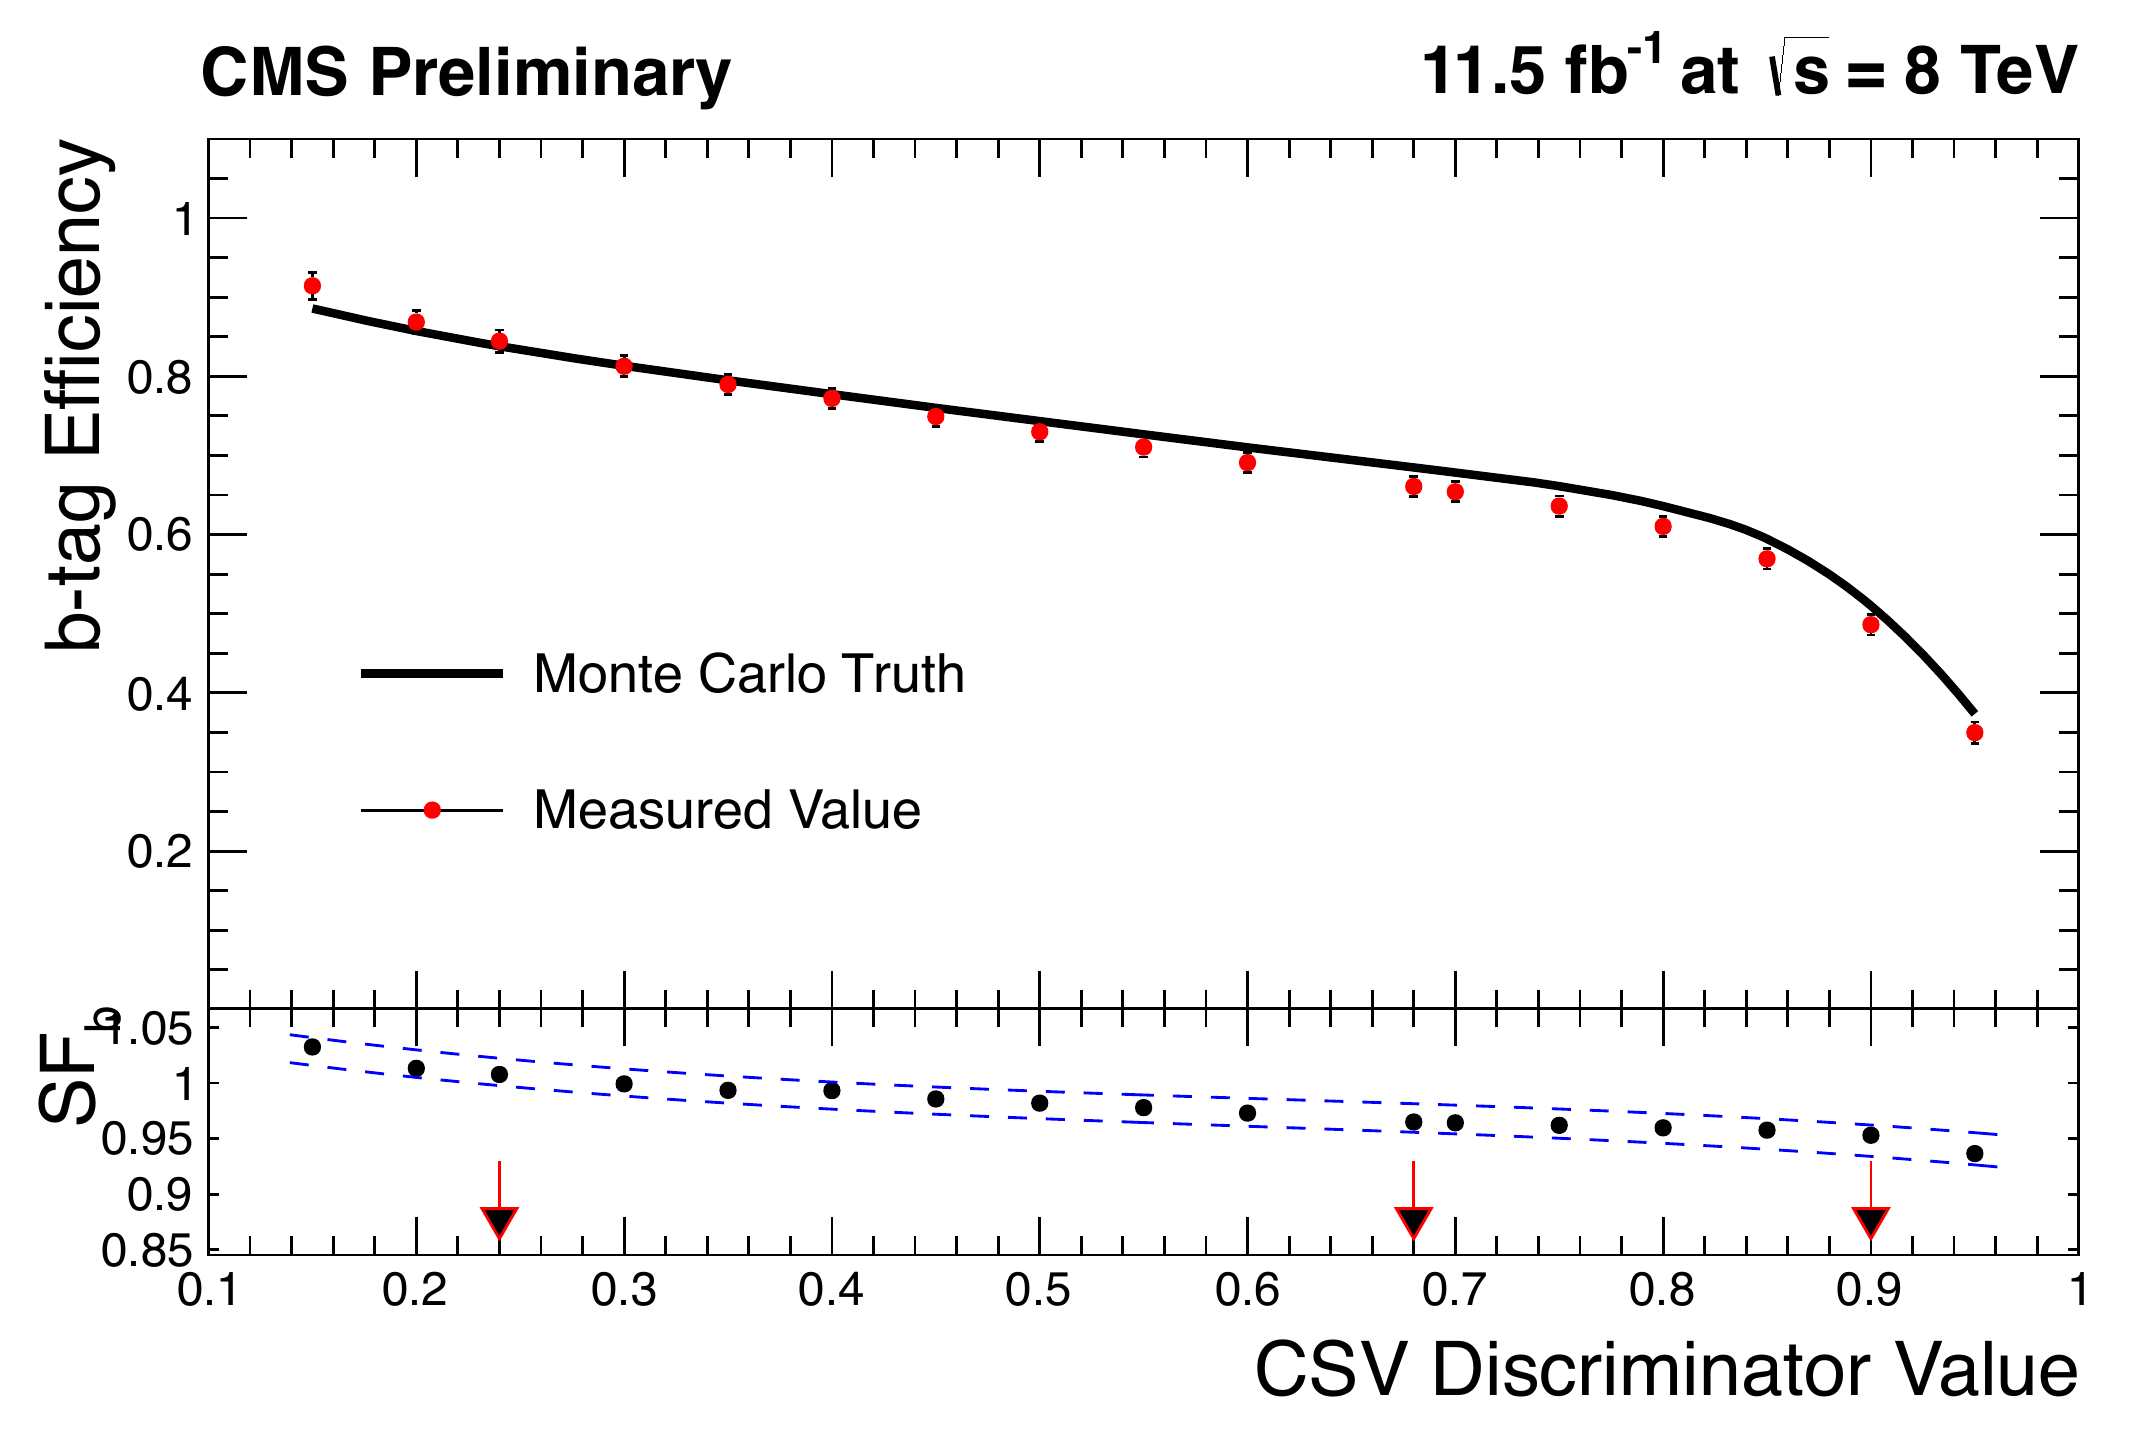
\includegraphics[width=0.6\textwidth]{plots/RECO/bTagEfficiency.png}\\

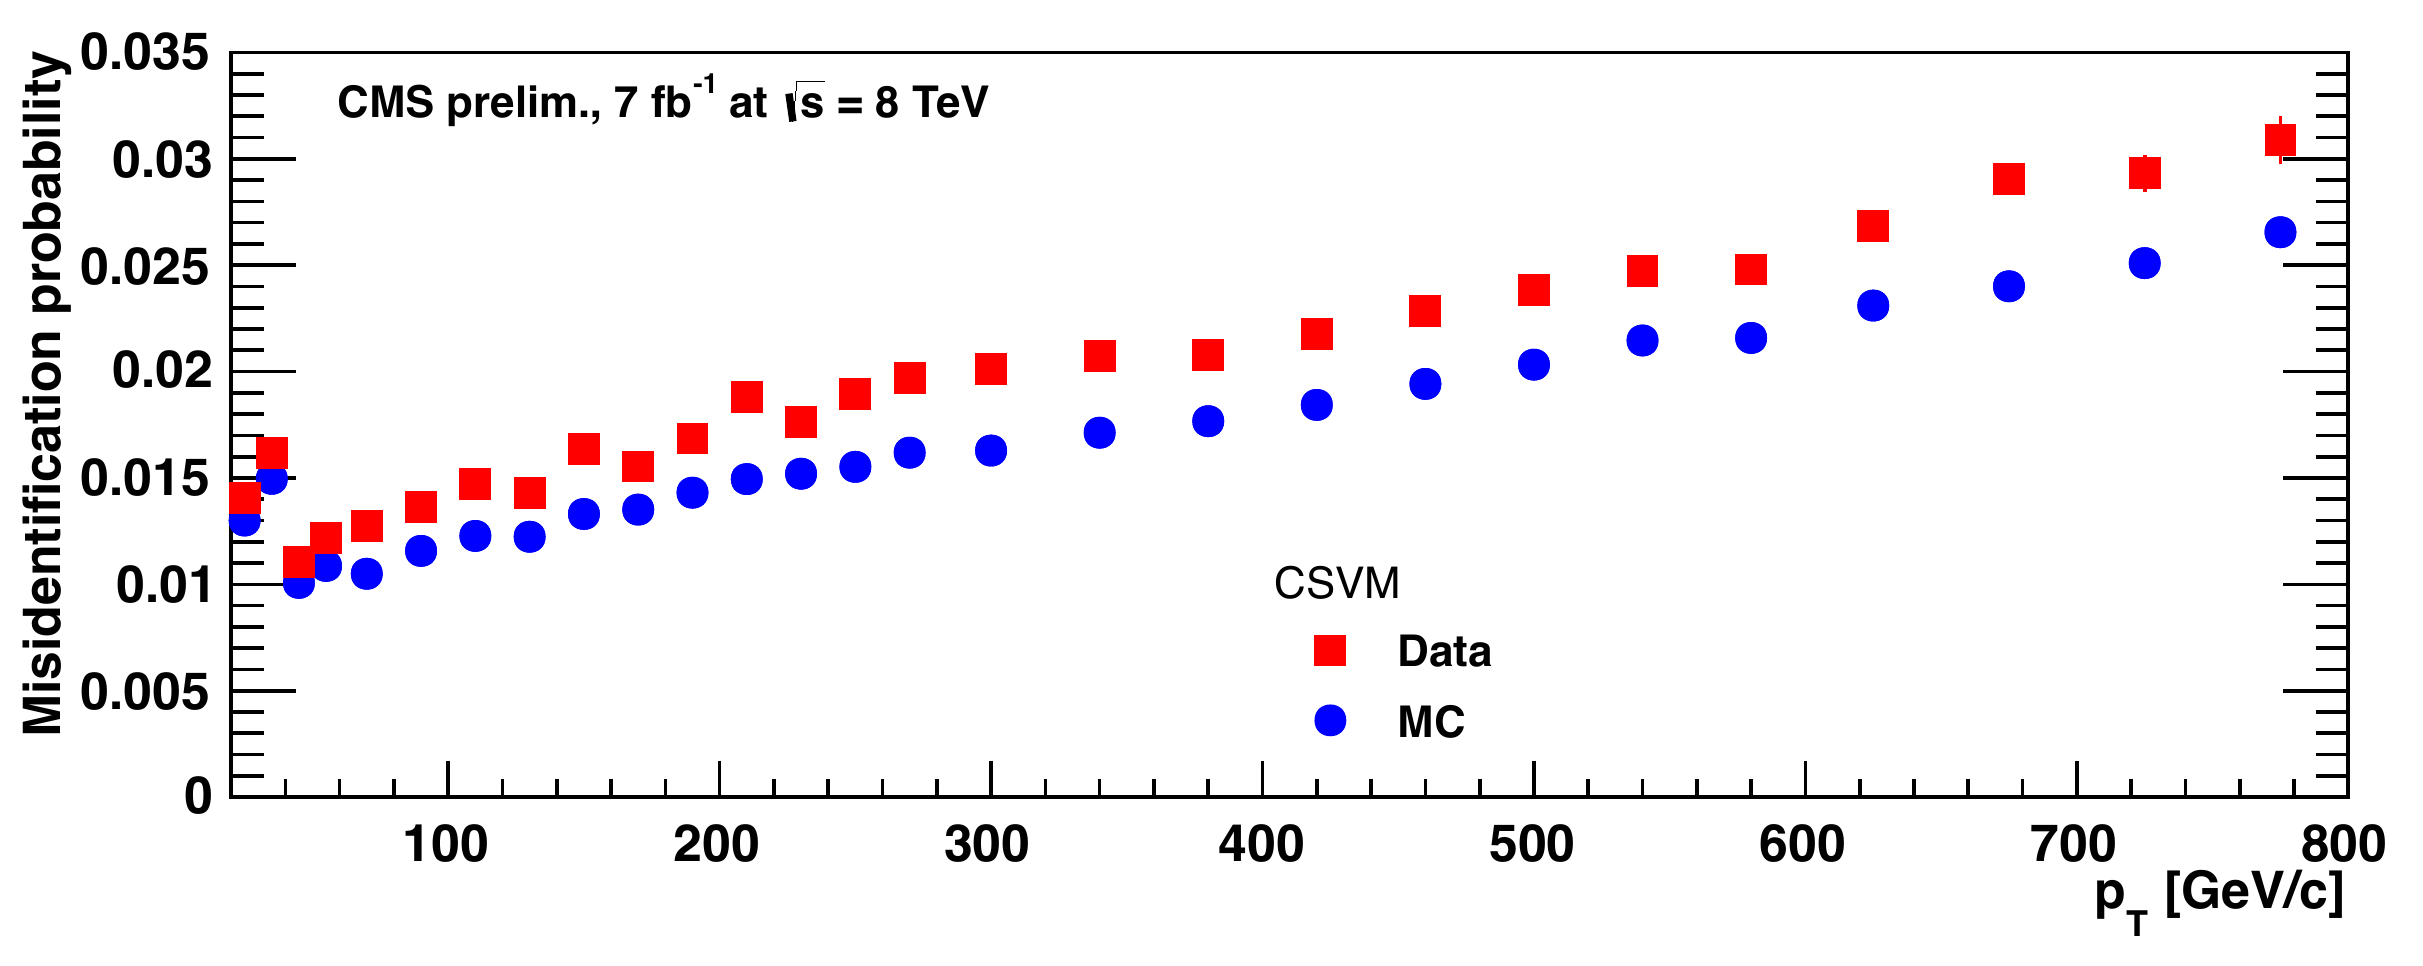
\includegraphics[width=0.6\textwidth]{plots/RECO/bTagMisID.png}\\

\caption{Performance of the CSV b-tagging algorithm. Shown is the identification efficiency as a function of the discriminator value (top) and the probability of misidentifying a jet originating from a light quark as a b-jet (bottom) as a function of \pt~\cite{CMS-DP-2013-005}. In the top figure, the scale factor between data and simulation is shown below the plot. The black arrows indicate three working points used in CMS.}
\label{fig:bTagging}
\end{figure} 

\subsubsection{Missing transverse energy}
As discussed in section~\ref{sec:variables}, \MET measures the imbalances of the energy depositions in the detector in the plane transverse to the beam direction. As this imbalance is the only experimental signature of this class of particles, a good \MET resolution is a key factor for the discovery of processes that include the production of new weakly interacting particles. 

Several algorithms have been developed in CMS to reconstruct \MET~\cite{7TeVMETPaper}. Calorimetric (Calo)~\METVec is calculated as the negative vector sum of the energy deposits in each calorimeter tower. Muons deposit only very small amounts of energy in the calorimeters, which are replaced by the measured muon \pt for this calculation. A further correction is introduced in the track-corrected (TC)~\METVec. For well reconstructed tracks, the track measurement is more precise than the measurement of a hadron's energy in the HCAL. Therefore, for tracks not associated with an electron or  muon, the track measurement is used in the calculation of \METVec. The energy deposit in the calorimeter is excluded, based on a model of the calorimeter response, treating all hadrons as pions. In contrast to these subdetector-based approaches, the event description of the particle flow algorithm can be used to calculate \METVec. It is defined as the negative vector sum over the \pt vectors of all \textit{particle candidates}
\begin{equation}
 \METVec = - \sum\limits_{\textit{particle candidates}} \vec{p}_\mathrm{T}.
\end{equation}
Comparing the resolution for the \MET components in $x$ and $y$ direction, as shown in Figure~\ref{fig:METReso} for the data collected in 2011, PF \MET performs best of the three algorithms and is therefore used in this analysis.
\begin{figure}
\begin{center}
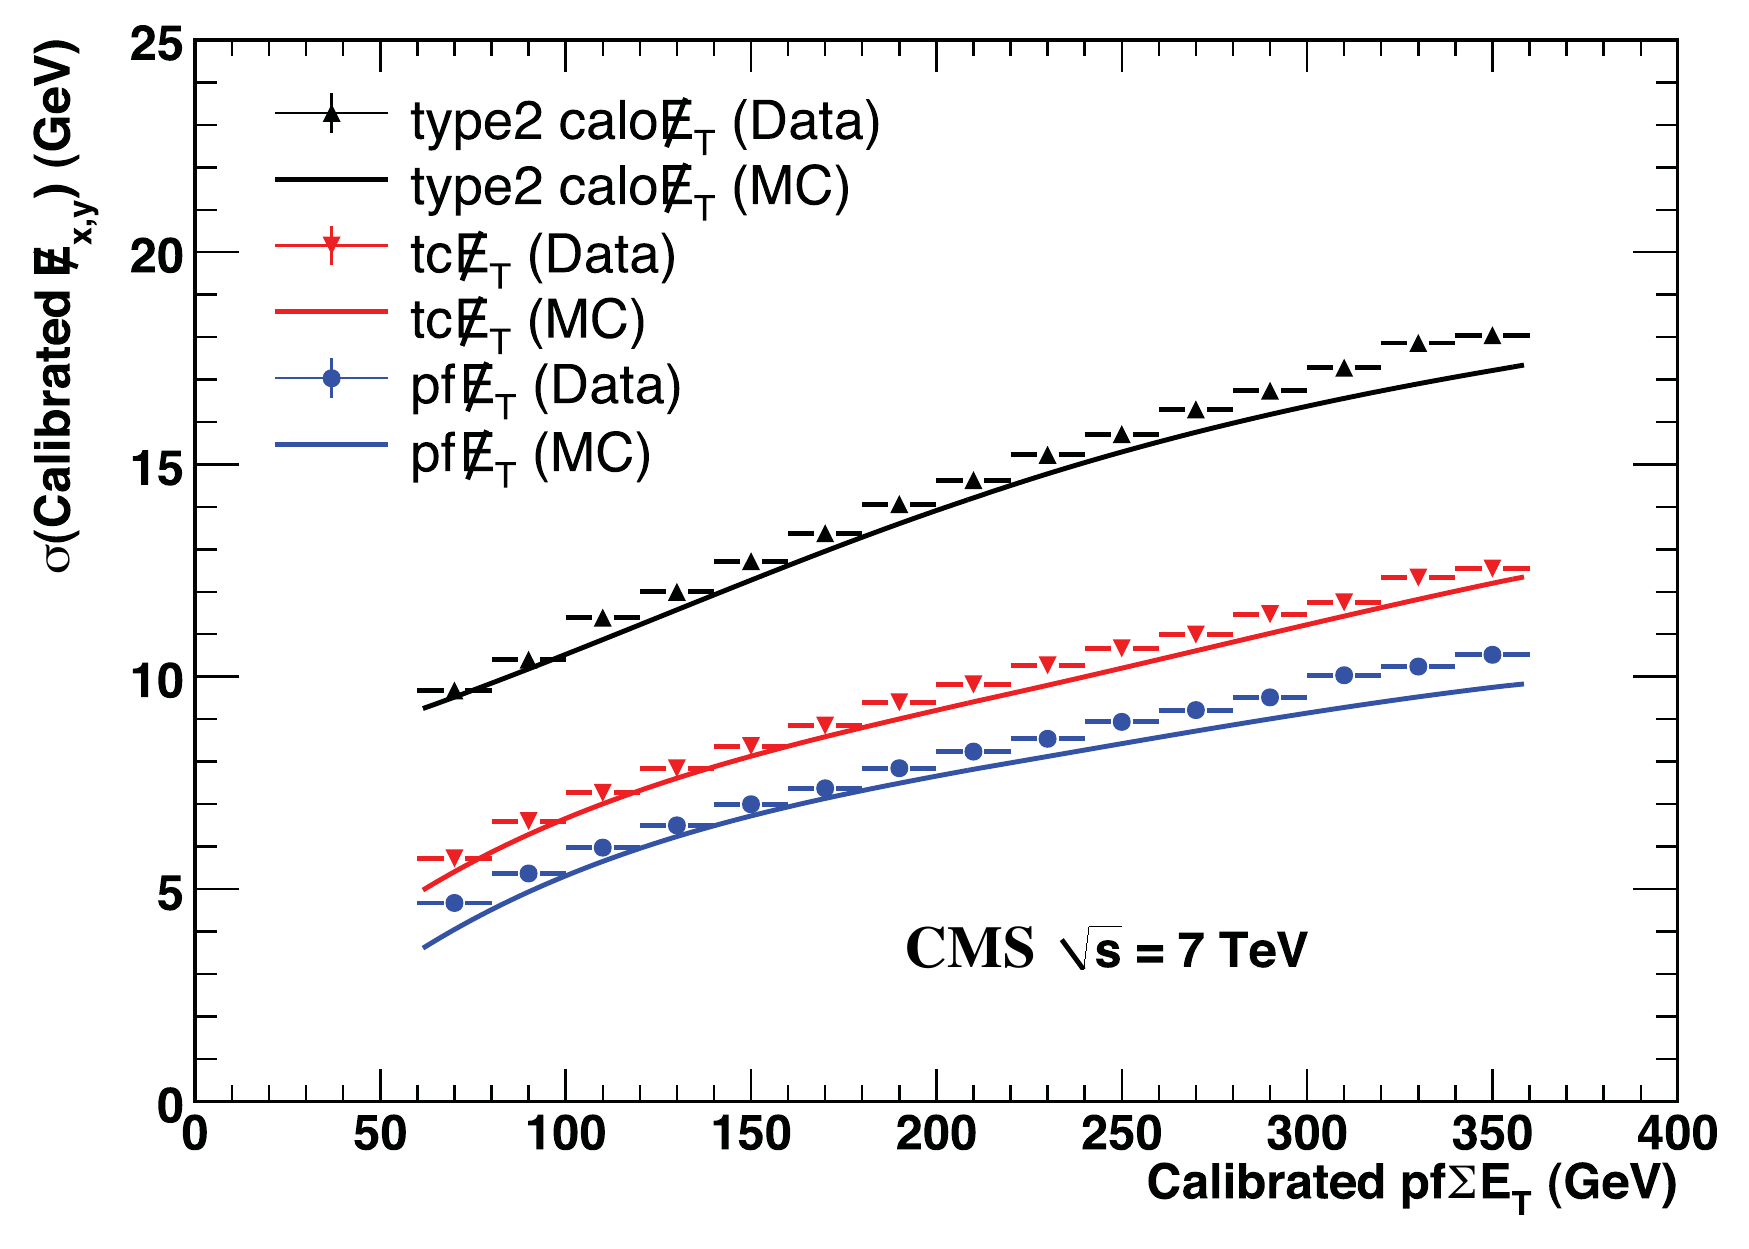
\includegraphics[scale=0.2]{plots/RECO/METResolution.png}
\caption{Calibrated \MET resolution as a function of the sum of the \Et of all particle flow candidates in an event. Shown are Calo \MET as black upward pointing triangles, TC \MET as red downward pointing triangles, and PF \MET as blue points~\cite{7TeVMETPaper}.}
\label{fig:METReso}
\end{center}
\end{figure}

Several corrections can be applied to the calculation of \MET. The $\textit{type-I}$ corrections propagate the corrections to the jet energy to the \MET calculation for all jets with \pt larger than $\unit{10}{\giga\electronvolt}$ and with less than 90\% of their energy deposited in the ECAL. The effects of pileup on the \MET reconstruction can be mitigated by applying $\textit{type-0}$ corrections, which are calculated on minimum bias events to parametrize the effects of such interactions on \MET. Further corrections can be applied to correct for modulations of the \MET in $\phi$~\cite{CMS-PAS-JME-12-002}. As this analysis searches for events with a large genuine \MET and is therefore not very sensitive to \MET introduced by resolution effect, none of these corrections are applied. However, $\textit{type-I}$ corrected PF \MET is considered as a cross check. 
\subsubsection{Lepton isolation}
While the lepton selection criteria described above are sufficient to reject backgrounds from particles misidentified as leptons, they do not suppress real leptons not originating from the primary interaction. As these are often produced in decays of bottom or charm quarks inside a jet, a more suitable criterion is to consider the amount of activity in the detector close to the lepton candidate, called lepton isolation. In this analysis, particle based isolation is used. For this the energy deposited by charged hadron, neutral hadron, and photon \textit{particle candidates} in a cone of $\Delta R = 0.3$ around the lepton is summed:
\begin{equation}
\text{Iso}^{text{uncorrected}} = \sum\limits_{\text{charged hadrons}} \pt + \sum\limits_{\text{neutral hadrons}} \pt + \sum\limits_{\text{photons}} \pt.
\end{equation}
The calculation of the isolation is distorted by pileup if PF candidates originating from pileup interactions lie within the cone and are counted in the isolation sum. This is easily remedied for charged hadrons, as those originating from a pileup vertex can be excluded from the calculation. For neutral hadrons and photons there is no track that can be associated to a vertex and a direct identification as pileup particles is not possible. Different approaches are pursued to correct for this contribution for electrons and muons. In both cases, an estimate for the contribution of neutral pileup is subtracted from the isolation sum, which changes to:
\begin{equation}
\text{Iso} = \sum\limits_{\text{charged hadrons from PV}} \pt + max(0, \sum\limits_{\text{neutral hadrons}} \pt + \sum\limits_{\text{photons}} \pt - \sum\limits_{\text{neutral PU}} \pt), 
\label{eq:iso}
\end{equation}
where $\sum\limits_{\text{neutral PU}} \pt$ is the estimated pileup contribution from neutral hadrons.
For electrons the correction is similar to the L1 offset correction for jets described above. As a measure of the pileup contribution in the isolation cone the median \pt density in the event $\rho$ is multiplied by the effective area of the electron in the detector, which is calculated in bins of $\eta$. The pileup correction is therefore defined as $\sum\limits_{\text{neutral PU}} E_T = \rho\cdot A^{\text{eff}}_{\text{electron}}$. For muons $\Delta \beta$ corrections are applied. Here, it is utilized that on average the contribution of neutral particles from pileup is half that of charged particles, leading to a correction defined as $\sum\limits_{\text{neutral PU}} E_T = \Delta\beta\cdot \sum\limits_{\text{charged PU}} E_T$ with $\Delta\beta = 0.5$. Because of the stochastic nature of these approaches, overcorrection is possible. Therefore, no negative contribution from neutral particles is allowed in equation~\ref{eq:iso}. For both electrons and muons the isolation sum divided by the lepton candidate's \pt (relative isolation) must not exceed  15\%. The choice of this requirement is discussed in more detail in section~\ref{sec:inclusiveSelection}.

 
\section{Event processing and datasets}
Events accepted by the HLT are reconstructed using the algorithms described above, implemented in the $\textbf{CMS}$ $\textbf{S}$oft$\textbf{w}$are (CMSSW) framework~\cite{PTDR1,SWGuideCMSSW}. While a first reconstruction is performed immediately after the data is recorded, making it available to analysis within a few days, the full dataset recorded by CMS in 2012 has been reprocessed in a second reconstruction with updated calibrations and detector alignment in the first months of 2013. The software version used for this purpose was \verb+CMSSW 5.3.7 patch6+. The events are stored in the $\textbf{A}$nalysis $\textbf{O}$bject $\textbf{D}$ata (AOD) format, which contains mostly high level objects, such as electrons and muons, and does not provide access to detailed detector information such as energy deposits, which are not of interest in many analyses. This allows to reduce the event size to $\unit{\approx0.1}{\mega\byte}$, compared to about $\unit{2}{\mega\byte}$ for the raw detector output. 

The data processing in this analysis is split into two parts. As a first step, the events in AOD format are processed utilizing the resources of the worldwide LHC computing grid~\cite{doi:10.1146/annurev-nucl-102010-130059,WLCG}, a system of cross-linked computing centres providing storage and computing capacities to the LHC experiments.  Datasets stored on grid sites can be accessed through the CMS remote analysis builder~\cite{CRAB}. At this stage, dilepton events are selected based on the identification criteria described above and the properties of the lepton pairs, together with other event characteristics, are stored. This is done with version \verb+V00-05-24+ of the \verb+SuSyAachen+ framework, which utilizes tools provided within the CMSSW framework, notably the physics analysis toolkit~\cite{PATNote}. All datasets used in this analysis have been processed using \verb+CMSSW 5.3.8 patch3+. Detector calibrations and alignment constants to be used in the processing of events in CMSSW are specified in so called \verb+Global Tags+. The tags used in this analysis are \verb+FT53_V21A_AN6+ for data and \verb+START53_V27+ for simulation.

The second part consists of all further analysis performed on the events selected in the previous processing. As the event size is much reduced, it can be performed using conventional desktop PCs. Throughout the event processing chain, the ROOT framework ~\cite{ROOT} for data analysis in particle physics is frequently used. In the final analysis steps, ROOT version \verb+5.34.21+ is used.  

\subsection{Primary datasets}

Events are sorted into different primary datasets based on the HLT decisions, grouping together events accepted by related triggers. As this allows for events to appear in several of theses datasets, precautions against double counting have to taken when combining different data streams in one analysis. The primary datasets most relevant to this analysis are \verb+DoubleElectron+, \verb+DoubleMu+, and \verb+MuEG+, containing, amongst others, events triggered by the different dilepton triggers. As auxiliary datasets, events from primary datasets triggered by \HT (\verb+HT+, \verb+JetHT+), single leptons (\verb+SingleElectron+, \verb+SingleMu+), and $\alpha_\mathrm{T}$ (\verb+HT+, \verb+HTMHT+) are used (see section~\ref{sec:trigger}). Each primary dataset is split into four subsets, labelled \verb+Run2012A+ to \verb+Run2012D+, each run defined by the run period of the LHC between two technical stops. The primary datasets are summarised in Table~\ref{tab:datasets}, where also the datasetpaths by which the samples can be accessed in the CMS bookkeeping system (DBS)~\cite{1742-6596-119-7-072001} is given.   

\begin{table}

\begin{center}
\begin{tabular}{c|c|c}
 Primary dataset & purpose & dataset \\
\hline 
\verb+DoubleElectron+ & Signal & \verb+/DoubleElectron/Run2012A-22Jan2013-v1/AOD+\\
 &  & \verb+/DoubleElectron/Run2012B-22Jan2013-v1/AOD+\\
 &  & \verb+/DoubleElectron/Run2012C-22Jan2013-v1/AOD+\\
 &  & \verb+/DoubleElectron/Run2012D-22Jan2013-v1/AOD+\\
\hline 
\verb+DoubleMu+ & Signal & \verb+/DoubleMu/Run2012A-22Jan2013-v1/AOD+\\
 &  & \verb+/DoubleMuParked/Run2012B-22Jan2013-v1/AOD+\\
 &  & \verb+/DoubleMuParked/Run2012C-22Jan2013-v1/AOD+\\
 &  & \verb+/DoubleMuParked/Run2012D-22Jan2013-v1/AOD+\\
\hline 
MuEG & Background prediction & \verb+/MuEG/Run2012A-22Jan2013-v1/AOD+\\
 &  & \verb+/MuEG/Run2012B-22Jan2013-v1/AOD+\\
 &  & \verb+/MuEG/Run2012C-22Jan2013-v1/AOD+\\
 &  & \verb+/MuEG/Run2012D-22Jan2013-v1/AOD+\\
\hline 
\verb+HT+, \verb+JetHT+ & trigger efficiencies & \verb+/HT/Run2012A-22Jan2013-v1/AOD+\\
 &  & \verb+/JetHT/Run2012B-22Jan2013-v1/AOD+\\
 &  & \verb+/JetHT/Run2012C-22Jan2013-v1/AOD+\\
 &  & \verb+/JetHT/Run2012D-22Jan2013-v1/AOD+\\
\hline 
\verb+HTMHT+ & additional trigger studies & \verb+/HTMHTParked/Run2012B-22Jan2013-v1/AOD+\\
 &  & \verb+/HTMHTParked/Run2012C-22Jan2013-v1/AOD+\\
 &  & \verb+/HTMHTParked/Run2012D-22Jan2013-v1/AOD+\\
\hline 
\verb+SingleElectron+ & additional trigger studies & \verb+/SingleElectron/Run2012A-22Jan2013-v1/AOD+\\
 &  & \verb+/SingleElectron/Run2012B-22Jan2013-v1/AOD+\\
 &  & \verb+/SingleElectron/Run2012C-22Jan2013-v1/AOD+\\
 &  & \verb+/SingleElectron/Run2012D-22Jan2013-v1/AOD+\\
\hline 
\verb+SingleMu+ & additional trigger studies & \verb+/SingleMu/Run2012A-22Jan2013-v1/AOD+\\
 &  & \verb+/SingleMu/Run2012B-22Jan2013-v1/AOD+\\
 &  & \verb+/SingleMu/Run2012C-22Jan2013-v1/AOD+\\
 &  & \verb+/SingleMu/Run2012D-22Jan2013-v1/AOD+\\

\end{tabular}


\caption{List of primary datasets used in the analysis. Additionally, the main purpose of the dataset and datasetpaths in DBS are given.}
\label{tab:datasets}
\end{center}
\end{table}



\subsection{Simulated datasets}
Simulated datasets of SM processes and SUSY models are used throughout the analysis in the design and validation of methods and the interpretation of the results in terms of potential signals. However, as the estimation of the SM backgrounds is performed almost exclusively on data, only a short overview over the simulation techniques is given. Dedicated methods are used for the different steps needed to achieve a complete model of the proton-proton interactions and the detector response. 
\subsubsection{Simulation of the physical processes}
\label{sec:MCGen}
Monte Carlo methods are used to generate events according to the properties of physical processes~\cite{PDG}.
At the beginning of the description of a process stands the calculation of the cross section for the given hard scattering of fundamental particles, using pertubation theory (see for example~\cite{HalzenMartin}). For many SM processes and also some BSM models, calculations in next-to-leading order (NLO) or next-to-next-to-leading order (NNLO) order in QCD have been performed. The automated calculations performed in the event generators used for the simulation in this analysis are however mostly restricted to leading-order (LO) accuracy. Scaling the events to calculated cross sections retains the higher order accuracy in the total cross section. Differential cross sections are, however, restricted to the the order the events are generated at.  

At a hadron collider, the total cross section for a process is given by the cross section for the hard scattering $\hat{\sigma}$, convolved with the parton density functions (PDFs) $f^p_i(x,Q^2)$, which give the probability that a parton $i$ with a fraction $x$ of the proton's momentum will take part in the interaction at the momentum scale $Q^2$. Considering all possible combinations of partons (three valence quarks, sea quarks and gluons), the total cross section is given by
\begin{equation}
\sigma (pp \rightarrow C)  = \sum\limits_{i,j} \int dx_1 dx_2 f^p_i (x_1,Q^2) f^p_j(x_2,Q^2) \hat{\sigma}(ij\rightarrow C).
\end{equation} 
The PDFs have to be inferred from data and have been studied in numerous fixed-target experiments and, most importantly, in deep-inelastic electron-proton scattering at the HERA collider~\cite{Aaron:2009aa}. Different approaches are used by several groups to parametrize the PDFs based on the available data. In the generation of simulated datasets for CMS analyses, the CTEQ6L1~\cite{Pumplin:2002vw} PDF set has been used. To study systematic effects introduced by the choice of PDF set, the NNPDF2.3~\cite{Ball:2012cx},MSTW2008~\cite{Martin:2009iq}, and CT10~\cite{Lai:2010vv} PDF sets are used. The dependence of the PDFs on the momentum scale is described by the DGLAP (Dokshitzer, Gribov, Lipatov, Altarelli, Parisi) evolution equations~\cite{Gribov,Altarelli:1977zs,Dokshitzer}, which are used to extrapolate them to the regime of the LHC. 

For most processes, Madgraph 5.1.3.30~\cite{Alwall:2011uj} is used to calculate the hard scattering process, together with additional emissions of partons as part of initial and final state radiation (ISR and FSR). The inclusion of these emissions at matrix element level allows for the modelling of the radiation of hard partons that are well separated from other final state particles. However, this treatment breaks down for soft or collinear emissions, which can in turn be described by dedicated parton shower models. For this, Pythia 6.4.22~\cite{Pythia} has been used for all samples relevant to this analysis. To achieve a consistent description of the parton shower, events are rejected in which the parton shower in Pythia produces jets in the phase space already covered by the emissions in Madgraph, using the MLM matching scheme~\cite{Hoche:2006ph}. 

The production of single top quarks is simulated using Powheg~\cite{Powheg,Alioli:2009je,Re:2010bp} at NLO in pertubative QCD for the leading jet. For these samples, a similar matching of the parton showers in Powheg and Pythia is applied.  
 
The hadronization of colour-charged particles produced in the hard scattering or the parton shower is a non-pertubative process which can only be described by phenomenological models. The $\textit{string fragmentation}$ model, as used in Pythia, is based on the idea of colour strings connecting the colour-charged particles. The energy stored in the strings increases linearly with the distance between the  particles, until the string breaks and a $q\bar{q}$ pair is created, allowing for the formation of colour-singlets. These singlets may in turn break, until there is no longer enough energy available to continue with this process~\cite{Pythia}. The hadronization model, as well as the description of the underlying event and multi-parton interactions, has to be tuned to best describe existing data. For all samples used in this analysis, the tune $Z2^{*}$~\cite{Field:2011iq} is used. 

The decays of $\tau$ leptons are simulated with the dedicated software Tauola~\cite{Jadach1993361}, which includes polarization, spin correlations effects and intermediate hadron resonances. 

To simulate the effects of pileup, several simulated proton-proton interactions from a sample containing mostly soft QCD processes are added to the simulated events, including pileup interactions with a time distance to the event of $\unit{\pm50}{\nano\second}$ to emulate the effects of out-of-time pileup. The distribution of the number of additional interactions used in the simulation had to be estimated before the data taking and therefore differs from the one observed in the recorded dataset. This effect is corrected for, see section~\ref{sec:inclusiveSelection}.

\subsubsection{Simulation of the detector response}
A model of the CMS detector has been created using the GEANT4 toolkit~\cite{Agostinelli:2002hh}. It allows for a detailed description of the detector geometry and material budget and simulates the interactions of particles with the detector material. It also models the propagation of the particles inside different materials, taking into account for example the magnetic field inside the CMS solenoid. The energy deposits created by the interactions of the particles with the detector are converted into detector hits on which the full event reconstruction is performed. The simulation also includes a modelling of detector noise and dead readout channels.  

As this detailed simulation is quite time consuming, a fast simulation of the CMS detector has been developed~\cite{1742-6596-331-3-032049}. Trading some accuracy for large gains in processing time, the fast simulation is used in cases where large numbers of events have to be generated, for example in scans of the parameter space of a new physics model. Simplifications include for example an approximation of the tracker geometry, where the modelling of millions of individual modules has been replaced by thin cylinders of active and non-active material placed around the interaction point. A charged particle traversing these layers deposits some energy at the point at which it crosses an active layer with a predefined probability. Also, the reconstruction algorithms for tracks have been simplified. Similar approaches have been applied to all subdetectors. The simulation of detector noise is reduced. A decrease of processing time per event by two orders of magnitude is achieved. 

Simulated events are stored in the AODSIM data format, which is identical to the AOD format but also includes Monte Carlo truth information about the simulated particles and their production and decay history. This allows for a processing of simulated datasets with the same software as used in the analysis of data events. 
\subsubsection{Background datasets}
Possible background contributions in the analysis arise from all SM processes producing lepton pairs or one lepton with the possibility for other parts of their signature to be misidentified as a second lepton. The properties of these processes can be studied in simulation. Therefore, an extensive list of simulated processes is considered in the analysis. In many cases, processes are divided into different samples based on the different possible final states. This allows to produce larger sample sizes for decays with small branching fraction without having to generate enormous amounts of more abundant final states. The full list of considered processes is shown in Table~\ref{tab:MCSamples}. The samples have to be scaled according to the appropriate integrated luminosity, taking into account the number of generated events $N_{\text{events}}^{\text{gen}}$ and the cross section $\sigma$ of the process. The weight is then given by $w  = \frac{L\cdot \sigma}{N_{\text{events}}^{\text{gen}}}$. The top pair production is normalized to the cross section measured by CMS in the dileptonic decay channel~\cite{CMS-PAS-TOP-12-007}. Cross sections for the production and dileptonic decays of \W and \Z bosons have been calculated using FEWZ 3.1~\cite{Li:2012wna}, including corrections in N(N)LO in electronweak theory (QCD). MCFM 6.6~\cite{Campbell:2011bn} is used for the calculation of cross sections for diboson production. Cross sections for single top production have been calculated at approximately NNLO~\cite{Kidonakis:2012db}. Cross sections at NLO in QCD for triboson production have been calculated using aMC@NLO~\cite{Madgraph2}, while for $t\bar{t}$ production in association with one additional vector boson, MCFM 6.6 has been used~\cite{Garzelli:2012bn}. For  $t\bar{t}\W\W$ the cross section calculated by Madgraph is used. The cross section for top-pair production in association with a photon has been measured by CMS~\cite{CMS-PAS-TOP-13-011}.  
\begin{table}
\scriptsize
\begin{center}
\begin{tabular}{c|c|c|c|c|c}
category & process & generator &  cross section [pb] & processed events & weight\\
\hline 
$t\bar{t}$ & $t\bar{t} \rightarrow b\bar{b}\ell\nu \ell\nu$ & Madgraph & 23.84 & 11952631 & 0.04 \\
 & $t\bar{t} \rightarrow b\bar{b}q\bar{q}\ell\nu$ & Madgraph & 99.43 & 24913744 & 0.07 \\
 & $t\bar{t} \rightarrow b\bar{b}q\bar{q}q\bar{q}$ & Madgraph & 103.74 & 31172356 & 0.06 \\
\hline 
Drell-Yan & $Z/\gamma^{*} \rightarrow \ell\ell$ 10 \GeV $< m_{\ell} <$ 50 \GeV & Madgraph & 876.80 & 7132223 & 2.43 \\
 & $Z/\gamma^{*} \rightarrow \ell\ell$ $m_{\ell} >$ 50 \GeV & Madgraph & 3532.80 & 30000624 & 2.33 \\
\hline 
W & $W \rightarrow \ell\nu$ & Madgraph & 37509.00 & 55996720 & 13.26 \\
\hline 
WW,WZ,ZZ & $ZZ \rightarrow \ell\ell q\bar{q}$ & Madgraph & 2.45 & 1936727 & 0.03 \\
 & $ZZ \rightarrow \ell\ell\nu\nu$ & Madgraph & 0.36 & 954911 & 0.01 \\
 & $ZZ \rightarrow \ell\ell\ell\ell$ & Madgraph & 0.18 & 4789250 & $<$\,0.01 \\
 & $WZ \rightarrow l\nu \ell\ell$ & Madgraph & 1.06 & 2017979 & 0.01 \\
 & $WZ \rightarrow qq'\ell\ell$ & Madgraph & 2.32 & 3205557 & 0.01 \\
 & $WW \rightarrow \ell\nu \ell\nu$ & Madgraph & 5.81 & 1933235 & 0.06 \\
\hline 
single top & $t$ s-Channel & Powheg & 3.79 & 259961 & 0.29 \\
 & $t$ t-Channel & Powheg & 56.40 & 3746457 & 0.30 \\
 & $t$ tW-Channel & Powheg & 11.10 & 497658 & 0.44 \\
 & $\bar{t}$ s-Channel & Powheg & 1.76 & 139974 & 0.25 \\
 & $\bar{t}$ t-Channel & Powheg & 30.70 & 1935072 & 0.31 \\
 & $\bar{t}$ tW-Channel & Powheg & 11.10 & 493460 & 0.45 \\
\hline 
Other SM & $WWW$ & Madgraph & 0.08 & 220549 & 0.01 \\
 & $WW\gamma$ & Madgraph & 0.53 & 215121 & 0.05 \\
 & $WWZ$ & Madgraph & 0.06 & 222234 & 0.01 \\
 & $WZZ$ & Madgraph & 0.02 & 219835 & $<$\,0.01 \\
 & $t\bar{t}\gamma$ & Madgraph & 2.17 & 71598 & 0.60 \\
 & $t\bar{t}W$ & Madgraph & 0.23 & 196046 & 0.02 \\
 & $t\bar{t}Z$ & Madgraph & 0.21 & 210160 & 0.02 \\
 & $t\bar{t}WW$ & Madgraph & $<$\,0.01 & 217820 & $<$\,0.01 \\
\hline 
$t\bar{t}$ Systematics & $t\bar{t}$ & Madgraph & 227.00 & 6923750 & 0.65 \\
 & $t\bar{t}$, $m_{top} =$ 166.5 \GeV & Madgraph & 227.00 & 4469095 & 1.01 \\
 & $t\bar{t}$, $m_{top} =$ 169.5 \GeV & Madgraph & 227.00 & 5202817 & 0.86 \\
 & $t\bar{t}$, $m_{top} =$ 175.5 \GeV & Madgraph & 227.00 & 5186494 & 0.87 \\
 & $t\bar{t}$, $m_{top} =$ 178.5 \GeV & Madgraph & 227.00 & 4723379 & 0.95 \\
 & $t\bar{t}$, Matching scale up & Madgraph & 227.00 & 5393645 & 0.83 \\
 & $t\bar{t}$, Matching scale down & Madgraph & 227.00 & 5467170 & 0.82 \\
 & $t\bar{t}$, Factorization scale up & Madgraph & 227.00 & 5009488 & 0.90 \\
 & $t\bar{t}$, Factorization scale down & Madgraph & 227.00 & 5377388 & 0.84 \\

\end{tabular}
\caption{Simulated datasets used in the analysis. The samples are grouped by physics processes and information about the generator, the cross section of the processes, the number of processed events, and the resulting weight used to scale the simulation to the recorded luminosity are given.}
\label{tab:MCSamples}
\end{center}
\end{table}

For all occurrences of results based on simulation, the events are scaled by the trigger efficiency measured on data (see section~\ref{sec:triggerEffs}). If systematic uncertainties on the simulation are shown, they include uncertainties on the jet energy scale, trigger efficiencies, cross sections, and the pileup reweighting. In the case of $t\bar{t}$, the events are reweighted to correct for differences in the distribution of the \pt of the top quarks between data and simulation~\cite{TopReweighting}. For this process the systematic uncertainties additionally include uncertainties introduced by this reweighting as well as uncertainties on the choice of the matching and factorization scale in the generation of the events. Notably, no uncertainties on the parton distribution functions are considered. Also, many smaller uncertainties on the modelling of physics objects are not considered. Therefore, the shown uncertainty presents a lower bound on the actual systematic uncertainty on the simulation. As the background contributions are estimated from data in this analysis, neither the imperfect knowledge of these uncertainties nor their size affect the results.

To correctly reproduce the effects of pileup in the simulated samples, the simulated events have to be reweighted based on the number of simultaneous interactions in the events. For simulation the distribution of these interactions is precisely know, for data it has to be inferred from the observed events, taking into account the total inelastic proton-proton interaction cross section. The effects of the reweighting procedure are illustrated in Figure~\ref{fig:PU}, where the distribution of the number of reconstructed vertices is shown for an inclusive selection of \EE and \MM events (see section ~\ref{sec:inclusiveSelection}). The left side shows the distribution before reweighting. The difference between data and simulation is clearly visible, but is almost completely compensated by the reweighting, except for very low numbers of reconstructed vertices. However, this affects only a tiny fraction of the data sample.

\begin{figure}[htbp]
\centering
\begin{minipage}[t]{0.49\textwidth}
  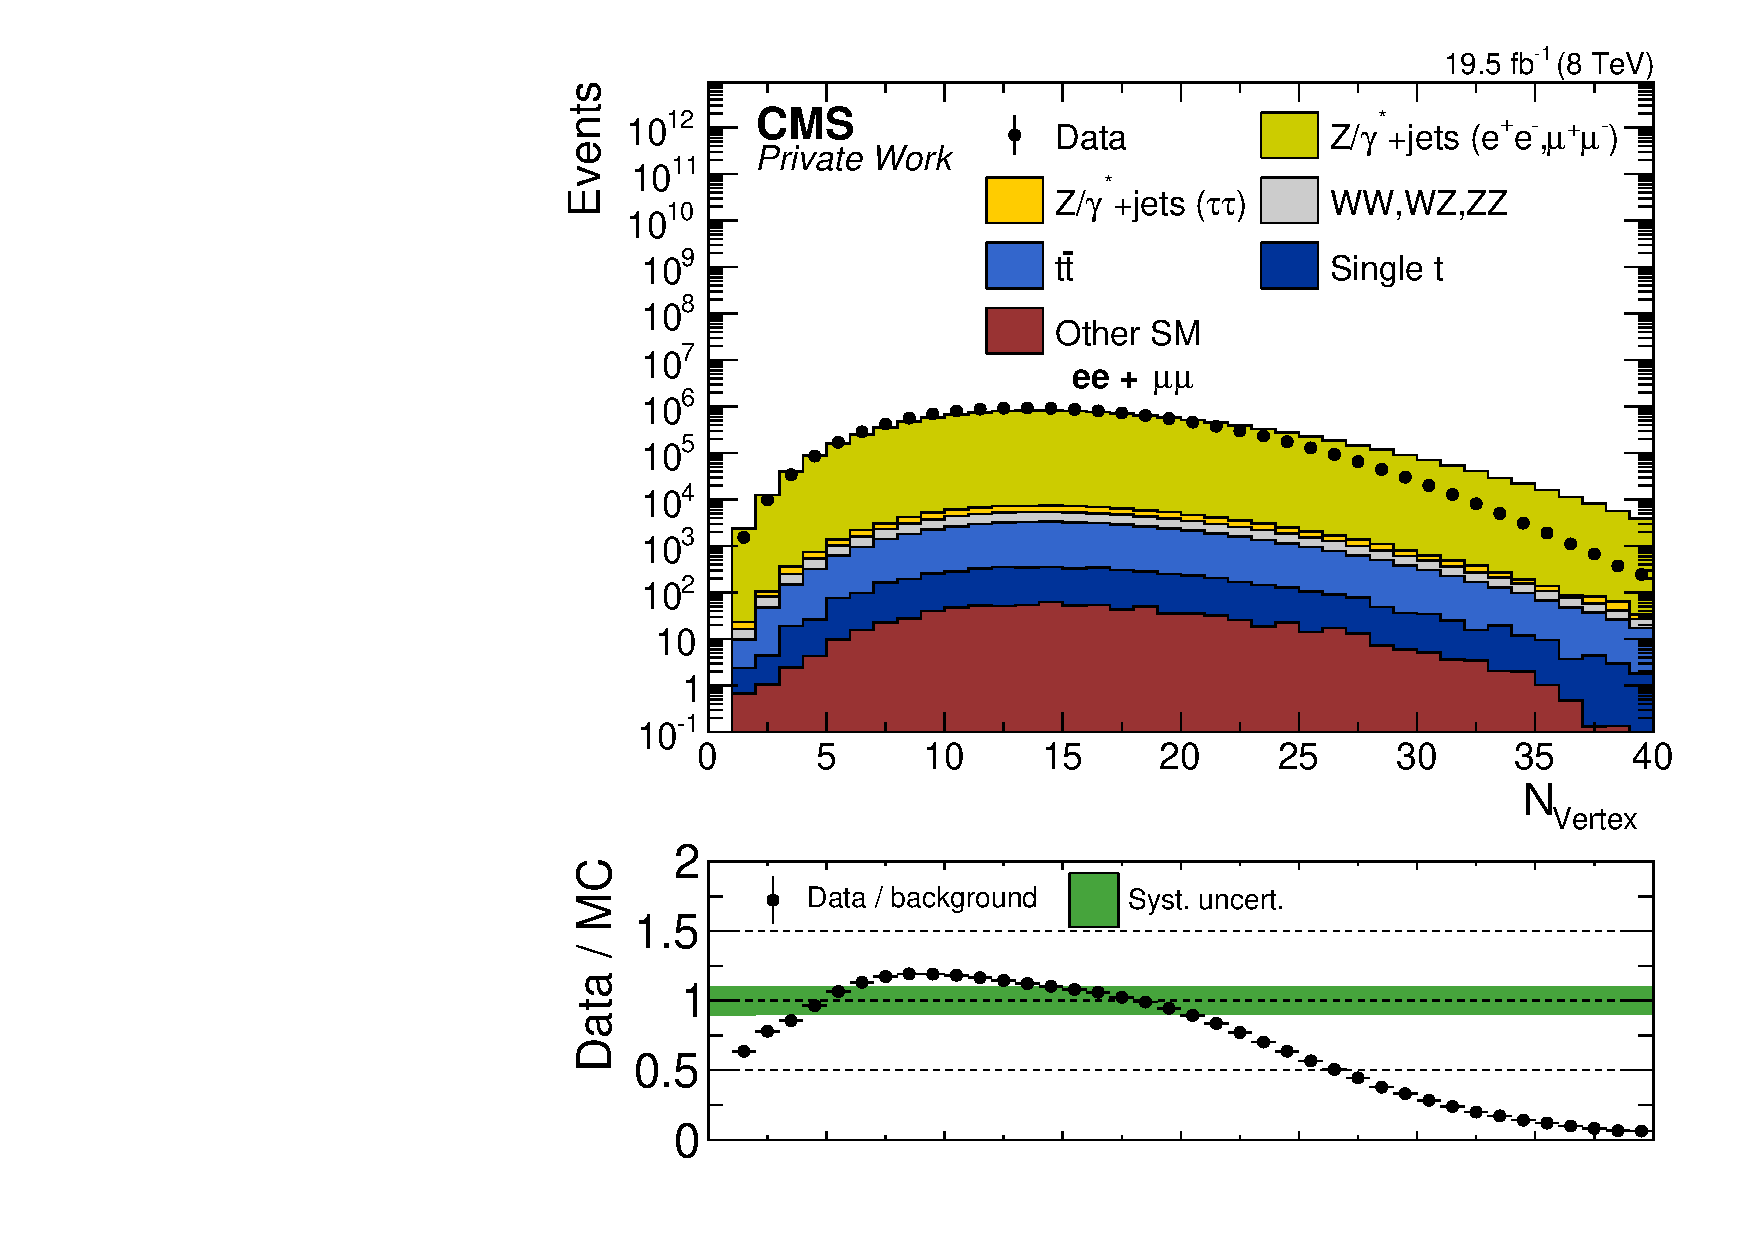
\includegraphics[width=\textwidth]{plots/SELECTION/Inclusive_nVtx_Full2012_SF_TopReweighted_NOPU.pdf}
\end{minipage}
\begin{minipage}[t]{0.49\textwidth}
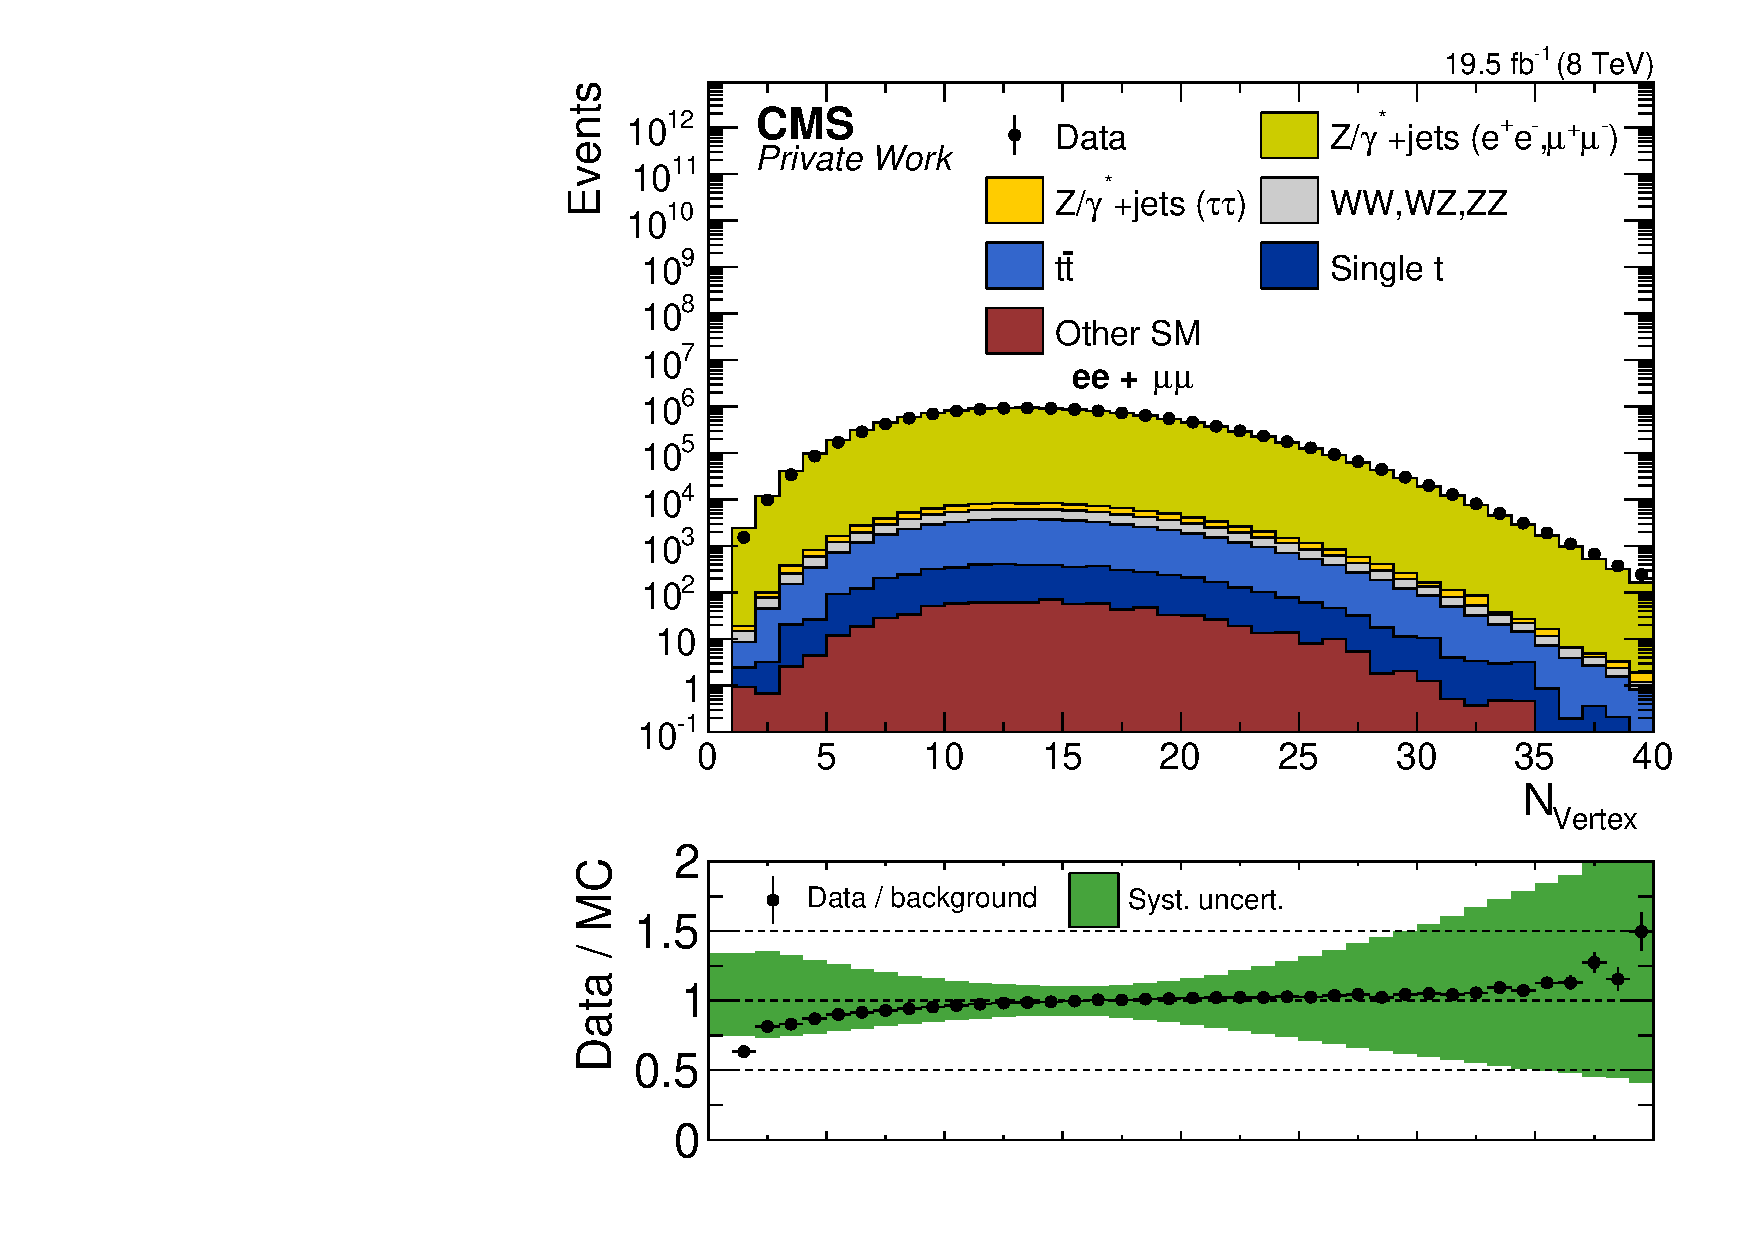
\includegraphics[width=\textwidth]{plots/SELECTION/Inclusive_nVtx_Full2012_SF_TopReweighted.pdf}
\end{minipage}
\caption{Distribution of the number of reconstructed vertices in an inclusive dilepton selection before (left) and after (right) pileup reweighting. The data is shown as black points. The different physical processes contributing to the sample are shown as stacked coloured histograms. Below the plots the ratio of data to simulation is shown is shown. The error bars on the black points include the statistical uncertainties of both data and simulation while the green band shows the systematic uncertainty on the simulation. }
\label{fig:PU}
\end{figure}   

\subsubsection{Signal datasets}
For simulated signals used in the analysis, initial squark pair production is simulated with Madgraph, including the emission of up to two additional partons at matrix element level. Sparticle decays and parton showers are generated with Pythia. The fast simulation of the CMS detector is used to model the detector response. Details of the physical models have been discussed in section~\ref{sec:models}.
\section{Event selection}
A series of selection criteria are applied to the events to select signal-like topologies and reduce the contributions from SM backgrounds to the final sample. Also, requirements are defined to select control regions enriched in certain SM processes for the purpose of background prediction and the validation of methods. Additionally, events are rejected that exhibit signs of detector noise or are otherwise not suited for analysis. 

\subsection{Event cleaning}
As a first step in the selection of reconstructed events, a series of quality requirements is applied. 
The quality of the data recorded by the CMS detector is assessed in several automated or manual steps, summarised as $\textit{Data quality monitoring (DQM)}$~\cite{DQM}. For each lumi section this results in a binary decision, flagging it as either $\textit{good}$ or $\textit{bad}$, accepting only those lumi sections for which all subdetectors were fully operational during data taking and no known problems occurred in the reconstruction of the events.

To reject non-collision events, vertex information is used. The presence of at least one primary vertex is required whose distance to the interaction point is less than $\unit{24}{\centi\meter}$ in $z$ direction and $\unit{2}{\centi\meter}$ in the $x$-$y$ plane. Also, the number of degrees of freedom, defined as~\cite{Chatrchyan:2014fea}:
\begin{equation}
n_{dof} = -3 + 2 \sum\limits_{i=1}^{N_{tracks}} w_i,
\end{equation}
is required to be greater than four.  

As it relies on the balance of all reconstructed objects, \MET is especially sensitive to distortions of the event reconstruction by noise or particles not originating from the proton-proton collisions. Several sources of these distortions have been identified during the data taking and filters have been developed in CMS to reject events matching their signatures~\cite{CMS-PAS-JME-12-002}. This includes filters for signal produced by interactions of the beam with gas molecules in the beam pipe or of protons in the beam halo with the LHC infrastructure, anomalous noise in the HCAL or ECAL, dead ECAL cells, calibration lasers mistakenly firing during collision events, or failures of the tracking algorithms. The effect of these filters on the tails of the \MET distribution in dijet events is shown in Figure~\ref{fig:METFilters}, where it can be seen that it is dominated by events that are rejected by the filters for \MET larger than $\unit{300}{\giga\electronvolt}$.
\begin{figure}
\begin{center}
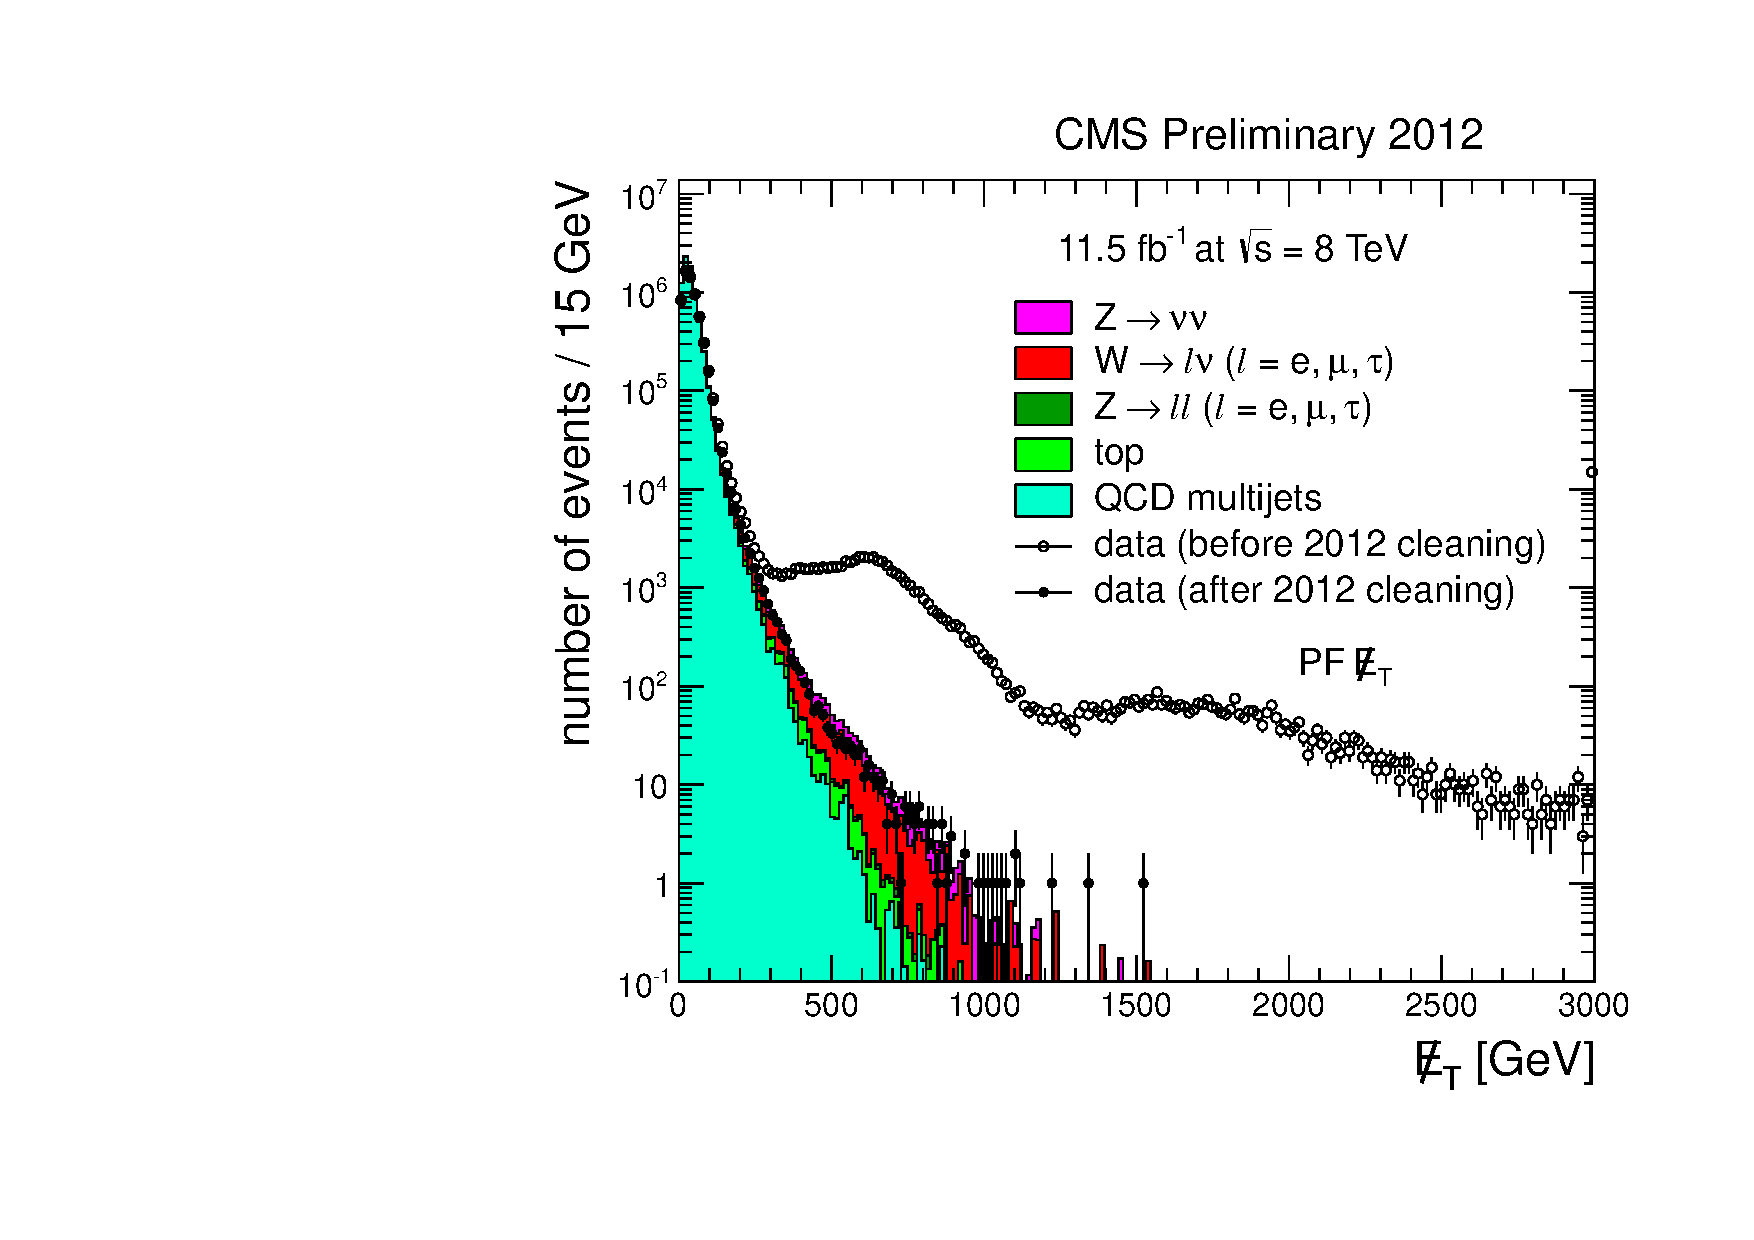
\includegraphics[scale=0.4]{plots/SELECTION/metFilter.pdf}
\caption{Distribution of \MET in dijet events in 2012 data. The open data points show all events, while the black points show the data after application of \MET filters. Simulated SM processes are shown as filled histograms.~\cite{CMS-PAS-JME-12-002}.}
\label{fig:METFilters}
\end{center}
\end{figure}


\subsection{Inclusive dilepton selection}
\label{sec:inclusiveSelection}
Events are selected containing two isolated electrons or muons with opposite electric charge, \pt larger than $\unit{20}{\giga\electronvolt}$, and $|\eta|$ smaller than 2.4. In the signal selection, only events with two same flavour (SF) leptons are considered. Events with opposite flavour (OF) leptons are used to estimate SM backgrounds. 

The choice of the isolation requirement of 15\% of the lepton \pt is illustrated on the left side of Figure~\ref{fig:isolation}, where the distribution of the relative isolation is shown for the trailing lepton in \ttbar simulation. Using the MC truth information the sample is split into prompt leptons originating from \W boson decays, leptons originating from heavy flavour hadron decays inside b-quark jets, and jets misreconstructed as leptons. The prompt leptons are concentrated at very low values, but a long tail extends to much higher values. The leptons from heavy flavour decays are less well isolated, with a broad maximum of the distribution between 0.5 and 1. Misreconstructed leptons are spread more evenly between high and low values of isolation. The cut value of 0.15 allows for a strong suppression of non-prompt leptons while a high efficiency is retained for prompt leptons. The isolation efficiency as a function of the number of reconstructed vertices is shown on the right side of Figure~\ref{fig:isolation} separately for prompt electrons and muons in \ttbar and \zjets events. The efficiency in \zjets evens is about 5 percentage points higher compared to the more hadronic environment of \ttbar events. While the efficiency for electrons shows only a slight dependency on the number of vertices and therefore on the amount of pileup, for muons a more strong decrease of efficiency is observed for high numbers of vertices. However, for \ttbar events this is much less pronounced, as the efficiency is already diminished by the higher number of jets in this environment. The good separation of prompt and non-prompt leptons and the high efficiency for prompt leptons are therefore  retained even in the challenging conditions at the LHC. 

\begin{figure}[htbp]
\centering
\begin{minipage}[t]{0.49\textwidth}
  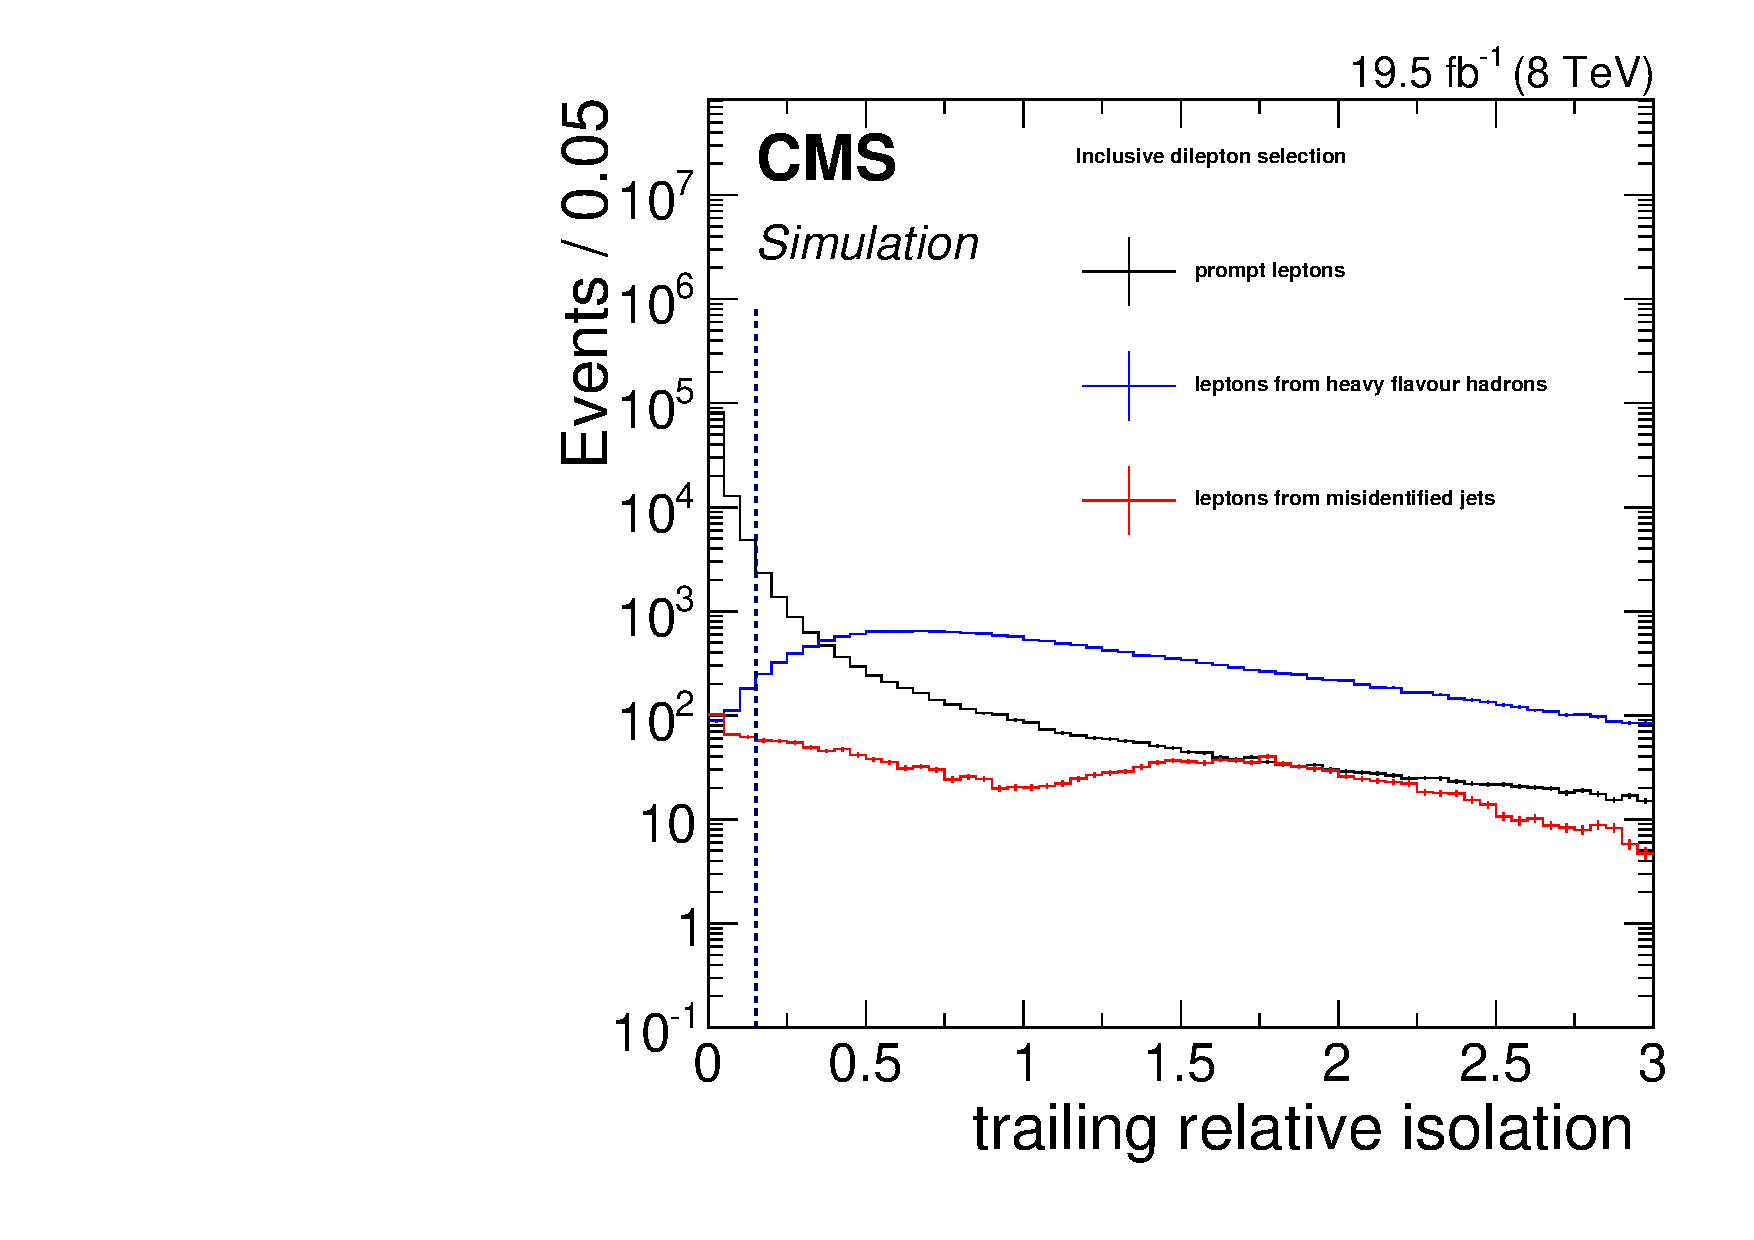
\includegraphics[width=\textwidth]{plots/SELECTION/iso_Inclusive_Full2012_TrailingIso_None_MC.pdf}
\end{minipage}
\begin{minipage}[t]{0.49\textwidth}
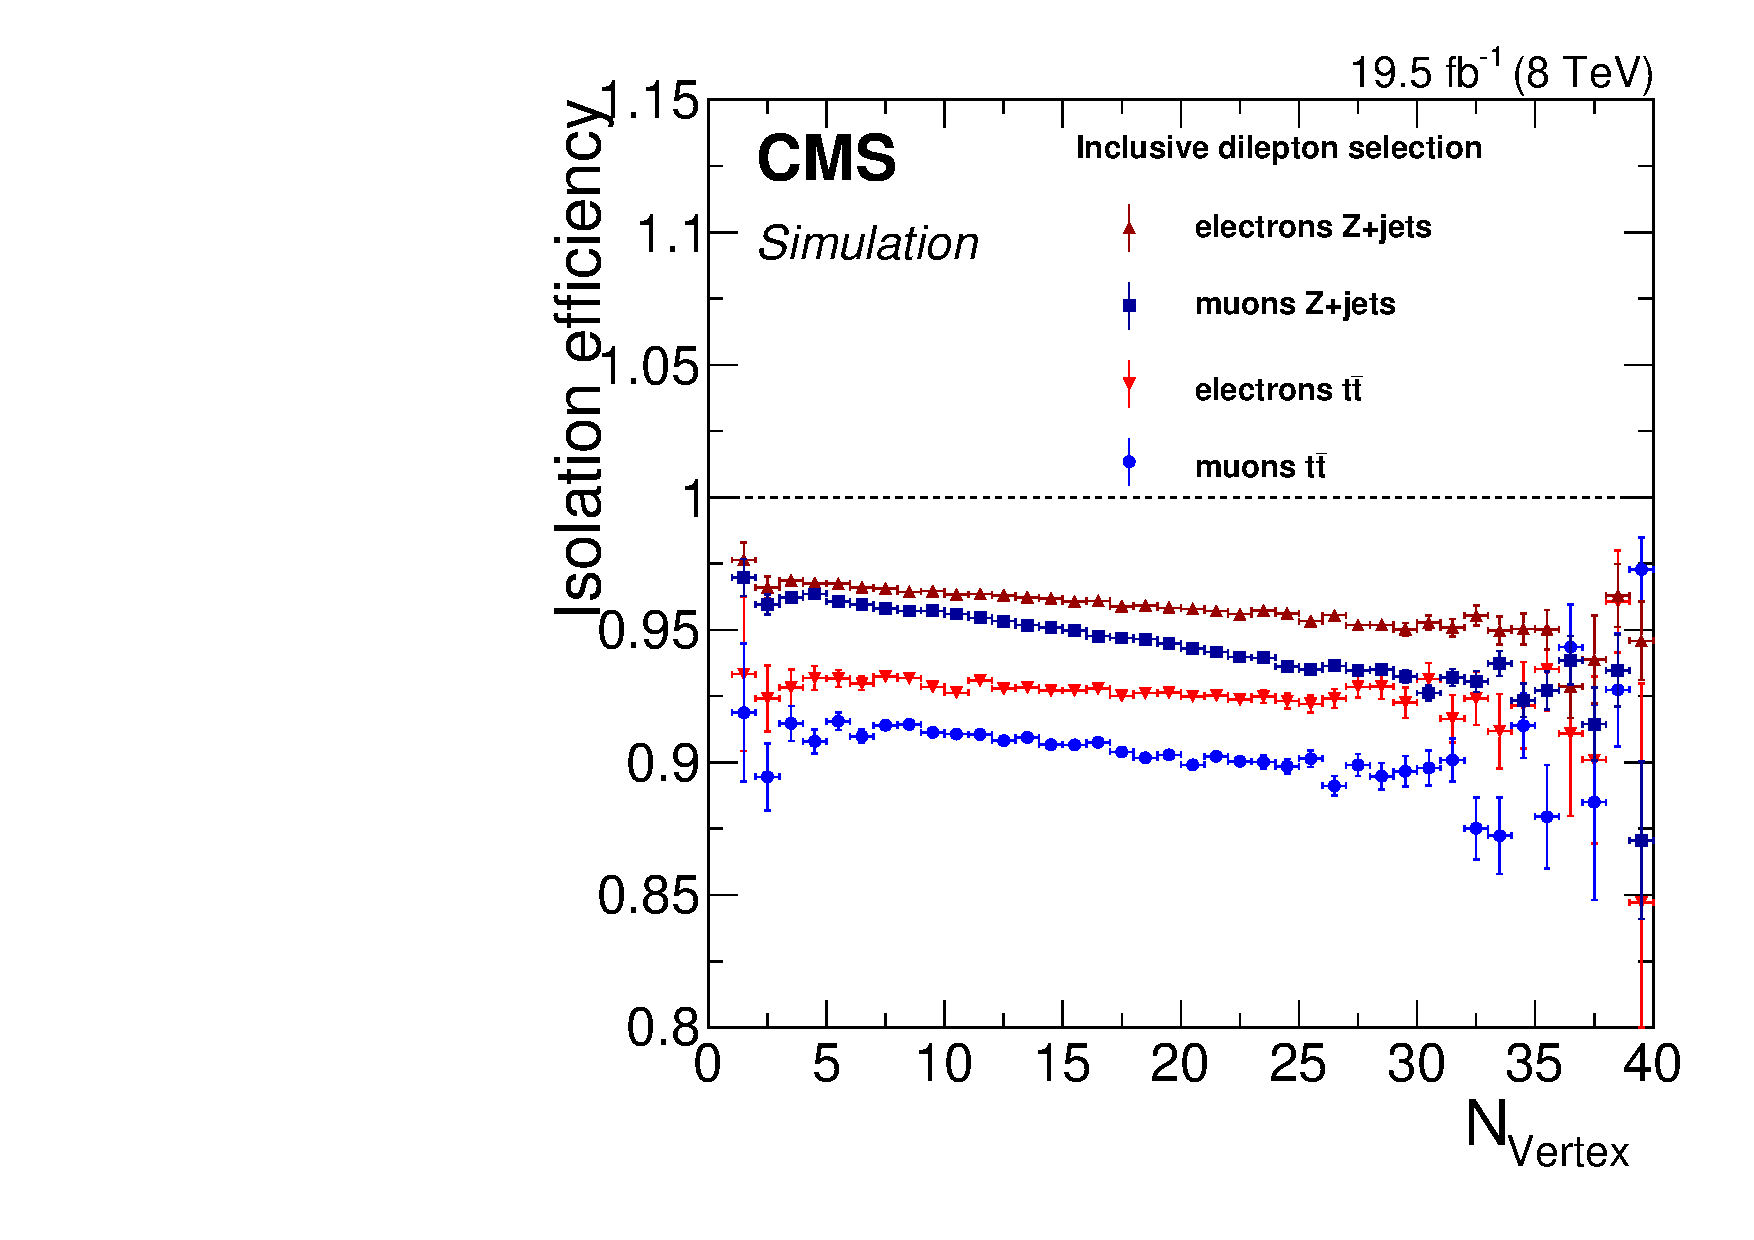
\includegraphics[width=\textwidth]{plots/SELECTION/isoEff_Inclusive_Full2012_nVtx_None_MC.pdf}
\end{minipage}
\caption{On the left, the distribution of the pileup corrected relative isolation of the trailing lepton for prompt leptons, leptons from heavy flavour decays, and misidentified jets in \ttbar simulation is shown. On the right side, the efficiency for a prompt lepton to pass the isolation requirement is shown as a function of the reconstructed number of vertices for both \ttbar and \Zjets simulation.}
\label{fig:isolation}
\end{figure}   

The \pt requirement is driven by the thresholds of the dilepton triggers, as discussed in Section~\ref{sec:triggerEffs}, while the $|\eta|$ restriction is imposed  by the coverage of the muon system. The acceptance for electrons could in principle be extended to $|\eta| =$ 2.5, but is chosen to be the same for both lepton flavours. Lepton pairs are required to be selected by the corresponding trigger, e.g. a pair of electrons has to have fired the dielectron trigger. If there is more than one pair of leptons fulfilling this basic requirements in one event, the pair with the largest scalar sum of lepton \pt is chosen. 

As the symmetry between lepton flavours is a key ingredient of the methods to estimate the backgrounds from SM processes, parts of the detector acceptance for which these symmetries are potentially violated are excluded:

As the efficiency to reconstruct electrons is reduced in the overlap region between the barrel and endcap detectors of the ECAL, the relative event yield for events with electrons with $|\eta|$ between 1.4 and 1.6 is reduced compared to those with muons in this range. This distribution of the $|\eta|$ of the leading lepton in \EE and  \MM events is shown in Figure~\ref{fig:cutJustification} (left), illustrating the greatly increased difference between the event yields for electrons and muons in the overlap region. Events containing a lepton with a pseudorapidity of $1.4<|\eta|<1.6$ are therefore rejected. Also, an increasing difference between electrons and muons can be seen for events were the leading leptons is in the endcap region of the detector. Therefore the event sample is split in two categories: $\textit{central}$, where both leptons are reconstructed with $|\eta| < 1.4$ and $\textit{forward}$, where at least one leptons has to be reconstructed with $|\eta| > 1.6$. The efficiency drop for muons around $|\eta| = 0.25$ is caused by the transition between different DT chambers in the muon system~\cite{CMS}.

Leptons with small spatial separation can interfere with each other's reconstruction and isolation. These effects are different for electrons and muons, which can be seen in Figure~\ref{fig:cutJustification} (right). The ratio of electrons to muons first rises for lower values of $\Delta R(\ell\ell)$ before dropping for values below $0.1$. The leptons are therefore required to be separated in $\Delta R(\ell\ell)$ by more than 0.3. Some differences between electrons and muons can also be observed for very high values of $\Delta R(\ell\ell)$, but they are less pronounced and this region is less populated.  

\begin{figure}[htbp]
\centering
\begin{minipage}[t]{0.49\textwidth}
  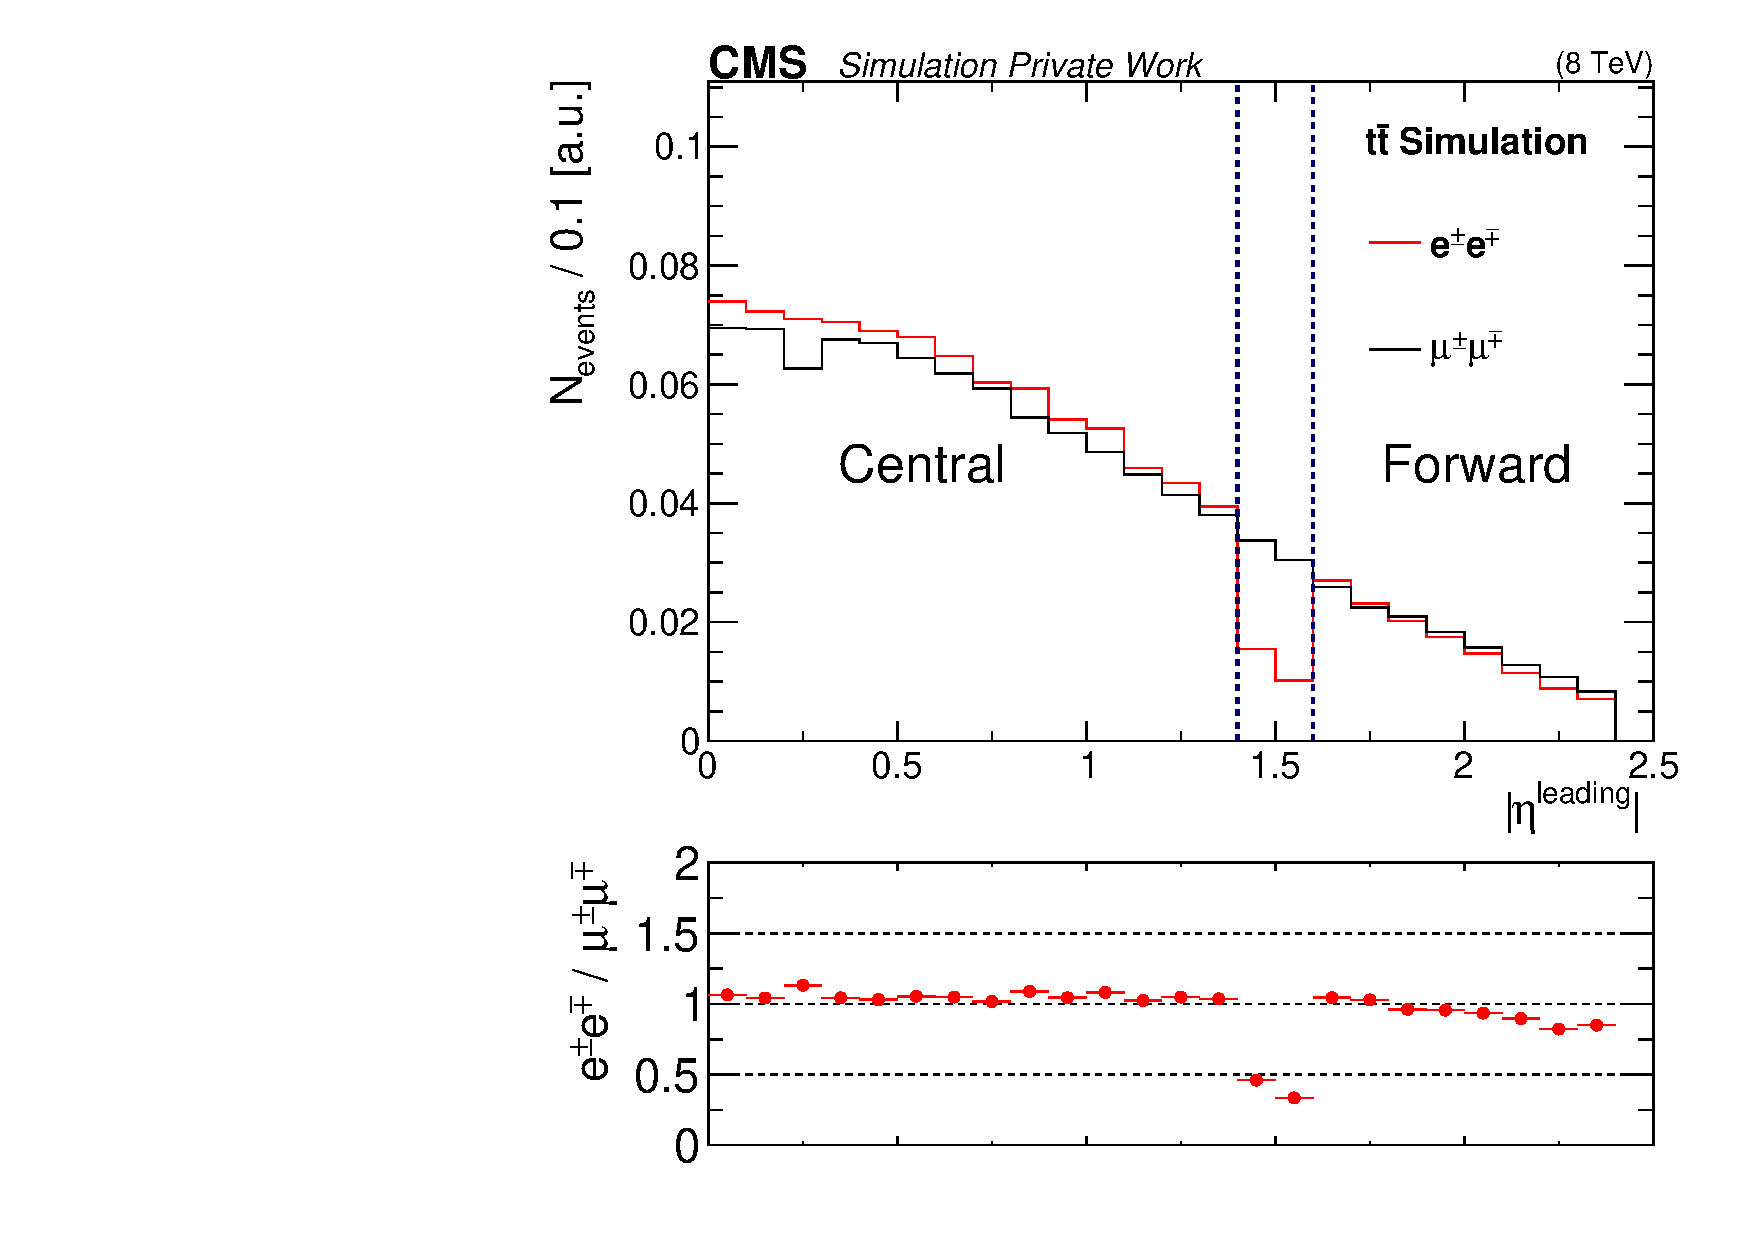
\includegraphics[width=\textwidth]{plots/SELECTION/gapJustification.pdf}
\end{minipage}
\begin{minipage}[t]{0.49\textwidth}
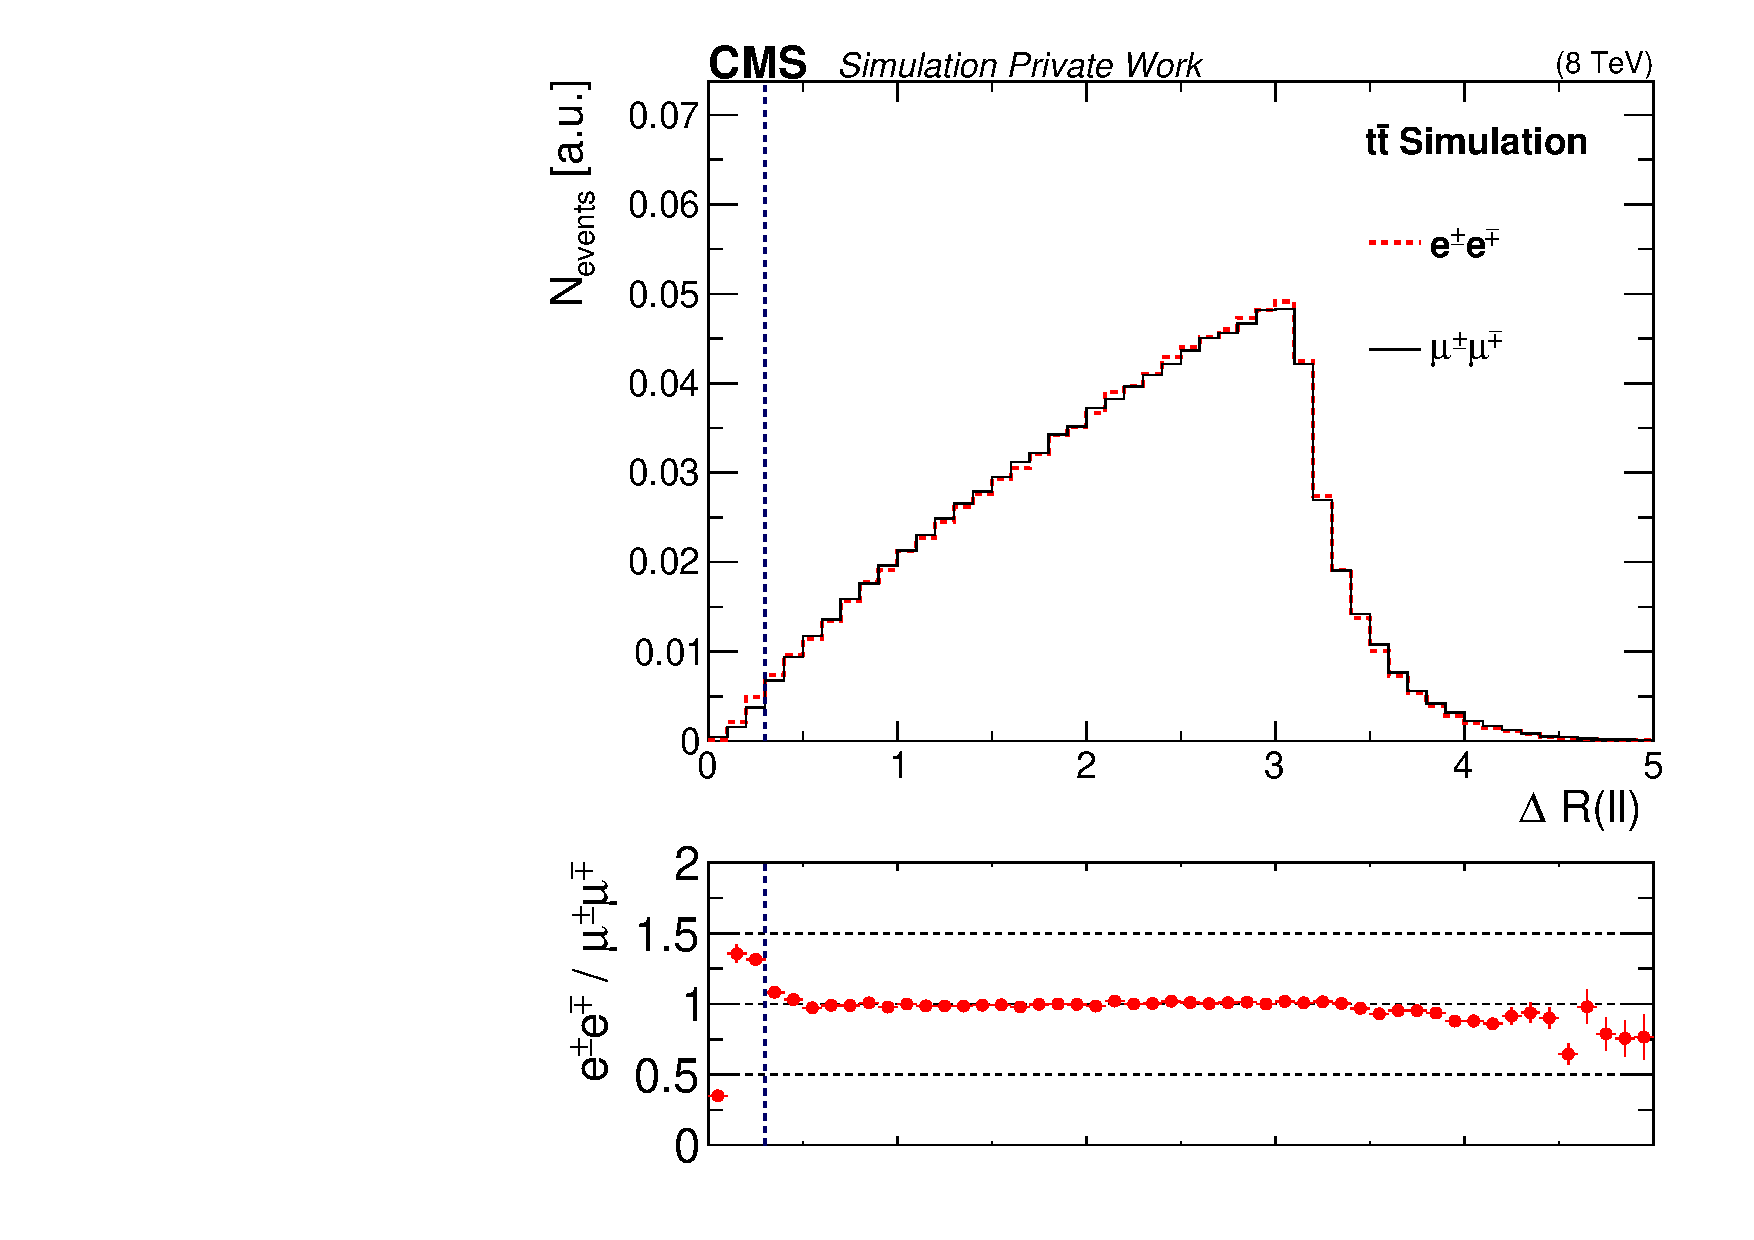
\includegraphics[width=\textwidth]{plots/SELECTION/dRJustification_eeVSmm.pdf}
\end{minipage}
\caption{Distributions of $|\eta|$ (left) and $\Delta R(\ell\ell)$ (right) for the leading lepton for \MM (black line) and \EE (red dashed line) events in a simulation of $t\bar{t}$ events. Both histograms have been normalized to an area of 1.}
\label{fig:cutJustification}
\end{figure}    

As an additional requirement, to avoid possible reconstruction problems events with low lepton momenta and to avoid contamination from dilepton production in the decay of the bottonium resonances, the dilepton invariant mass \mll is required to be greater than $\unit{20}{\giga\electronvolt}$. 


\subsection{Selections in \MET and jet multiplicity}
\label{sec:regions}
Three subsets of the event sample obtained with the inclusive dilepton selection are defined, resulting in samples enriched in different processes. The variables used in the definitions of these regions are \MET and the number of selected jets $N_{jets}$. The selections are illustrated in the plots of Figure~\ref{fig:sigRegionBG}, which also show the distribution of $t\bar{t}$ (left) and \Zjets (right) events in the \MET-$N_{jets}$ plane for SF leptons. 
 
The signal region, in which the search is performed, is defined by requiring either $N_{jets} \geq 3$ and $\MET > \unit{100}{\giga\electronvolt}$ or $N_{jets} \geq 2$ and $\MET > \unit{150}{\giga\electronvolt}$. This definition allows to select signal events for points in the parameter space where more energy is distributed to the jets and less to the invisible component of the signature and vice versa. At the same time the rejection of background events with both lower $N_{jets}$ and \MET is maintained. A control region dominated by flavour-symmetric processes is defined by selecting events with $N_{jets} = 2$ and $\unit{100}{\giga\electronvolt} < \MET < \unit{150}{\giga\electronvolt}$. 

To study lepton pairs produced via the Drell-Yan process and to obtain a high statistics sample of leptons for efficiency measurements, events with $N_{jets} \geq 2$ and $\MET < \unit{50}{\giga\electronvolt}$ are selected. The $N_{jets}$ requirement greatly reduces the statistics and the purity of this event sample. However, because of the large cross section of the Drell-Yan process, the event yield is still sufficient for the purposes of this analysis and Drell-Yan events dominate over those from $t\bar{t}$ production by two orders of magnitude. This allows to select events with kinematics close to those of the signal selection in terms of jet multiplicity.
\begin{figure}[htbp]
\centering
\begin{minipage}[t]{0.49\textwidth}
  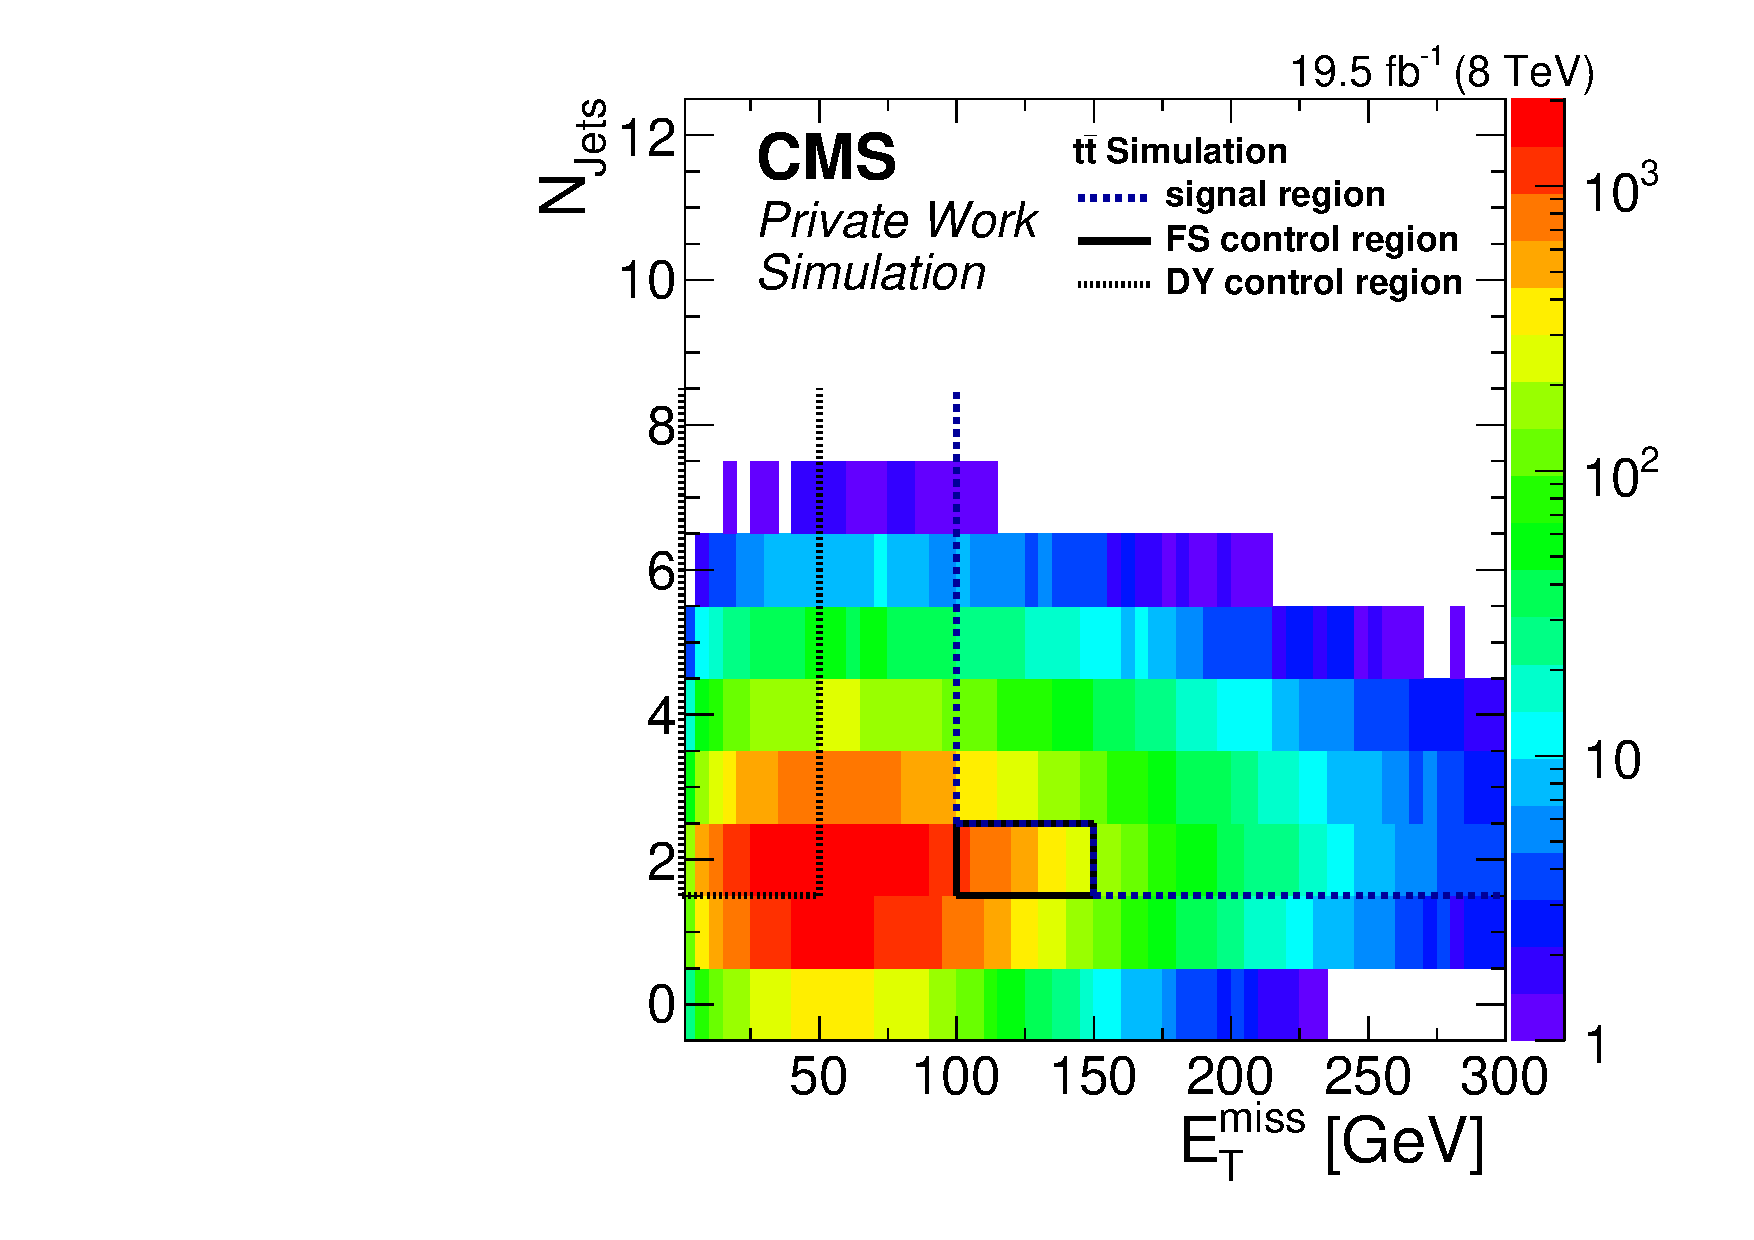
\includegraphics[width=\textwidth]{plots/SELECTION/metJetsScatter_ttbar.pdf}
\end{minipage}
\begin{minipage}[t]{0.49\textwidth}
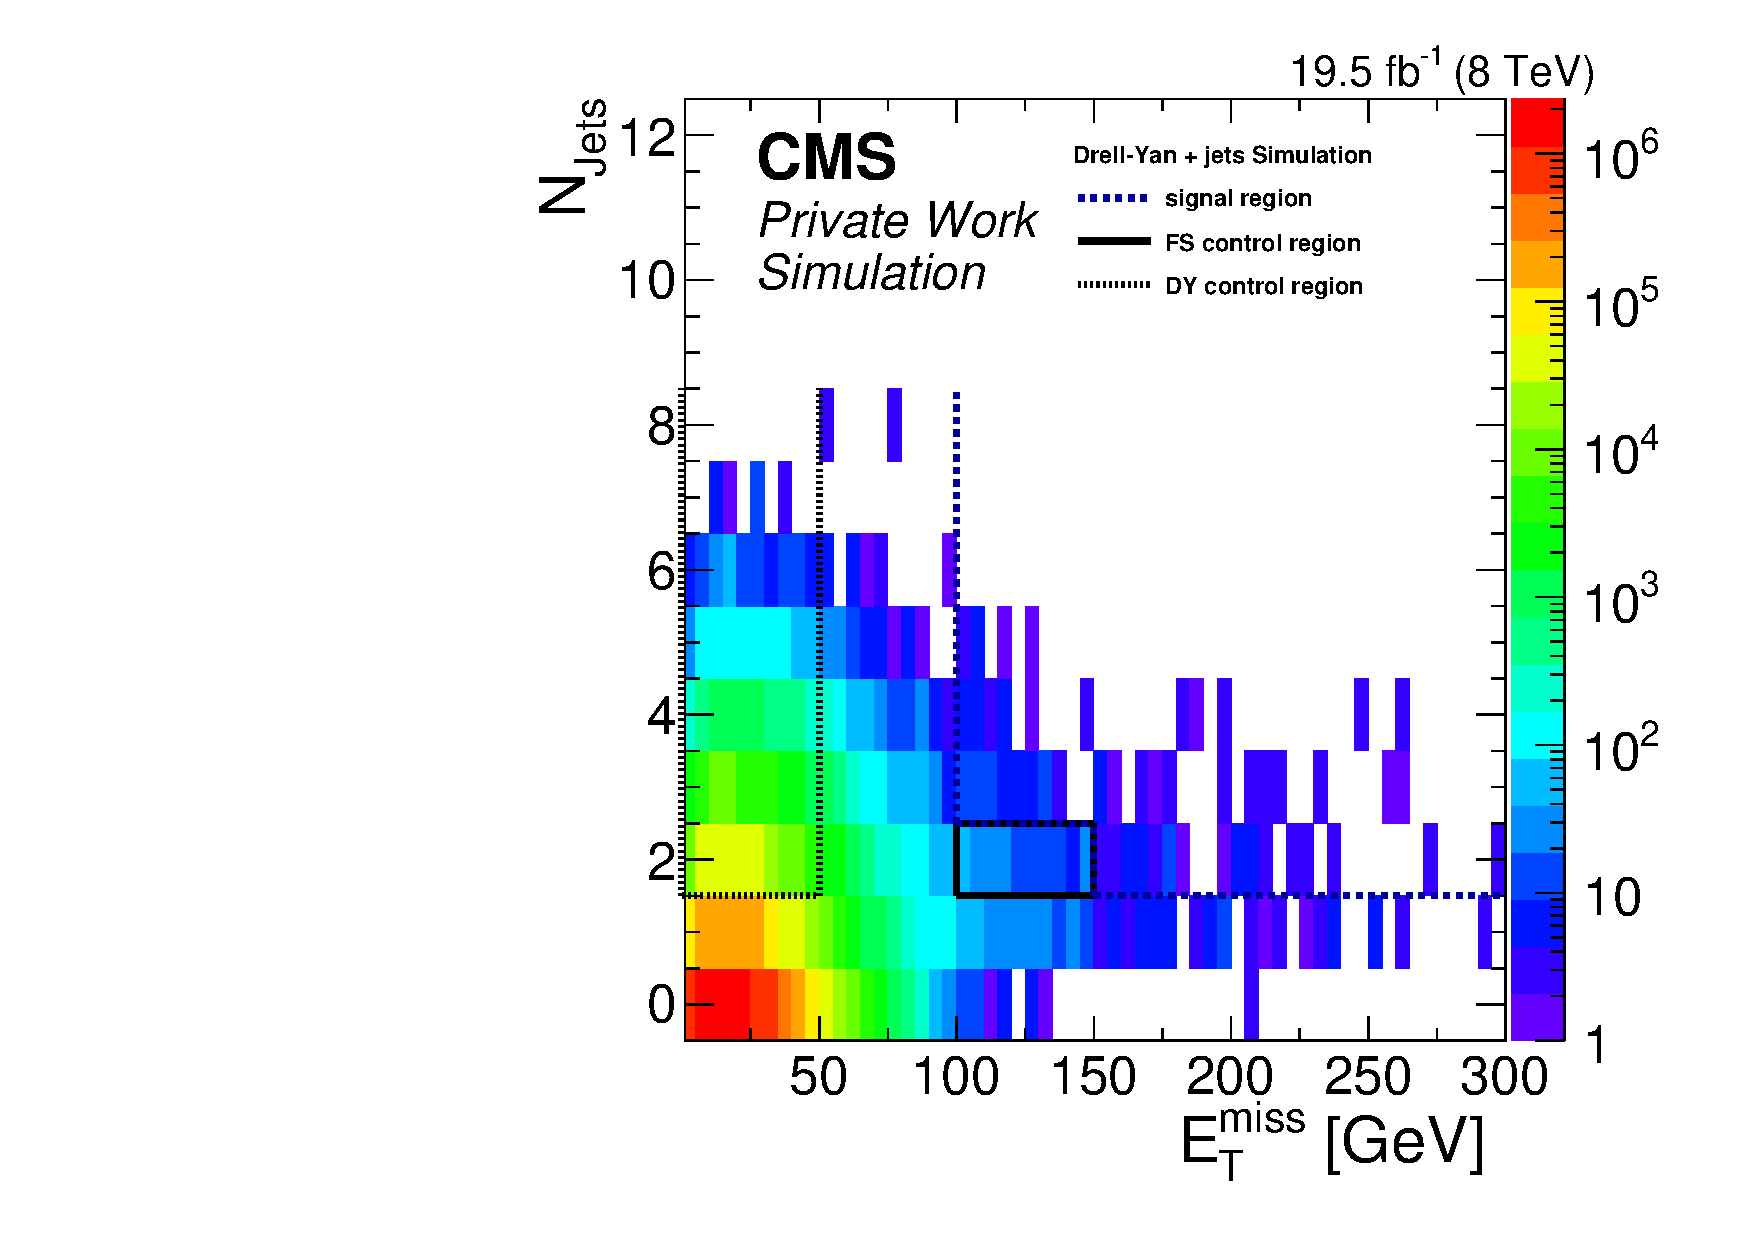
\includegraphics[width=\textwidth]{plots/SELECTION/metJetsScatter_DY.pdf}
\end{minipage}
\caption{Distribution of backgrounds events with SF leptons in the \MET-$N_{jets}$ plane for $t\bar{t}$ (left) and Drell-Yan (right) events from Simulation. The events are weighted according to the cross section of the process and the size of the generated event sample, assuming an integrated luminosity of \lumi. The three regions defined in the plane are indicated by lines. The central and forward dilepton selection are combined.}
\label{fig:sigRegionBG}
\end{figure}  
  
For comparison the same distributions are shown for two signal points from the models discussed in section~\ref{sec:models} in Figure~\ref{fig:sigRegionSignal}. On the left a point from the fixed-edge model with $m_{\sbottom} = \unit{550}{\giga\electronvolt}$ and $m_{\secondchi} = \unit{275}{\giga\electronvolt}$ (left) and on the right a point from the slepton-edge model with $m_{\sbottom} = \unit{500}{\giga\electronvolt}$ and $m_{\secondchi} = \unit{175}{\giga\electronvolt}$ are shown. For both signal points almost no events are observed with $\njets < 2$, which is expected because at least two b-jets are produced in each event. Compared to the backgrounds, a clear tendency towards higher \MET and \njets is observed. However, also contributions to two control regions are present, which are small compared to the background contributions. Overall, the chosen selection offers a good separation of signal and backgrounds.
\begin{figure}[htbp]
\centering
\begin{minipage}[t]{0.49\textwidth}
  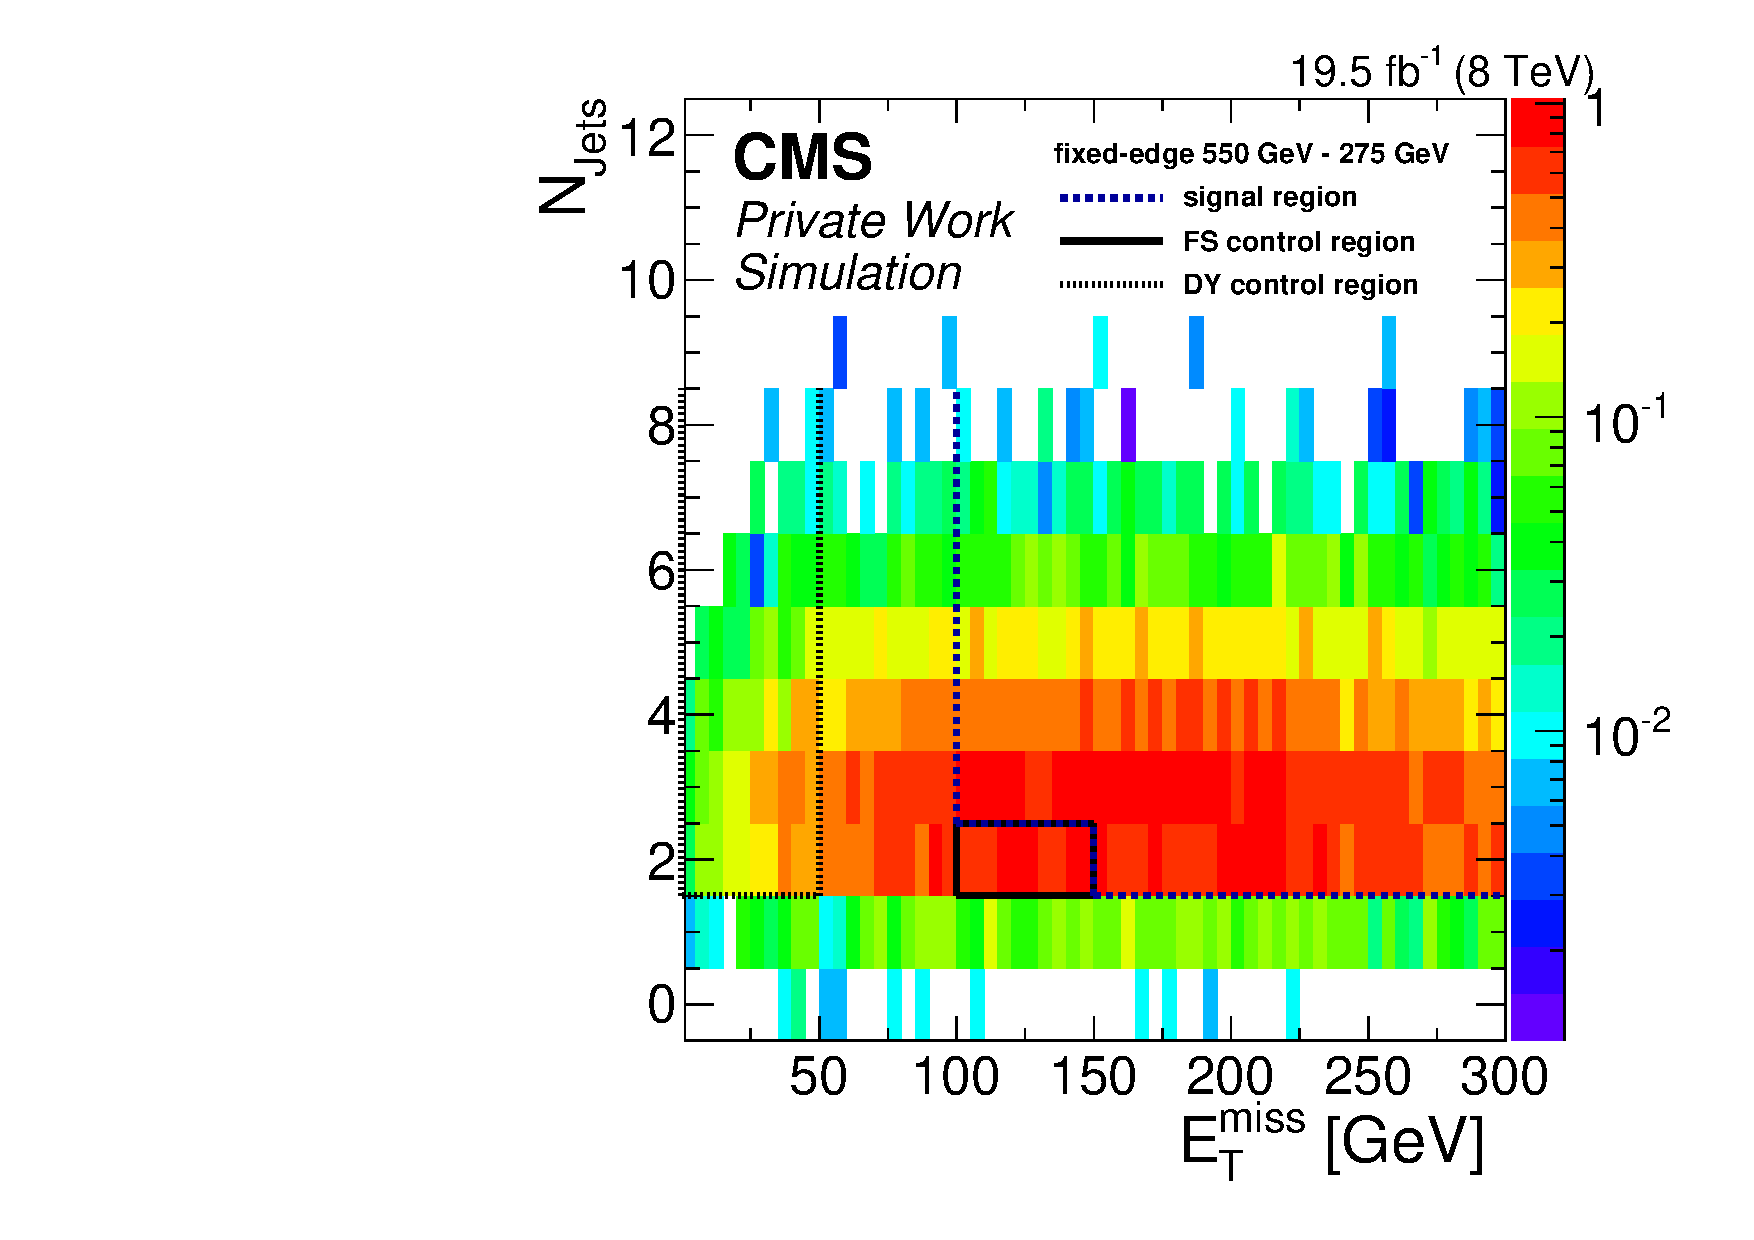
\includegraphics[width=\textwidth]{plots/SELECTION/metJetsScatter_SUSY_edge_550_275.pdf}
\end{minipage}
\begin{minipage}[t]{0.49\textwidth}
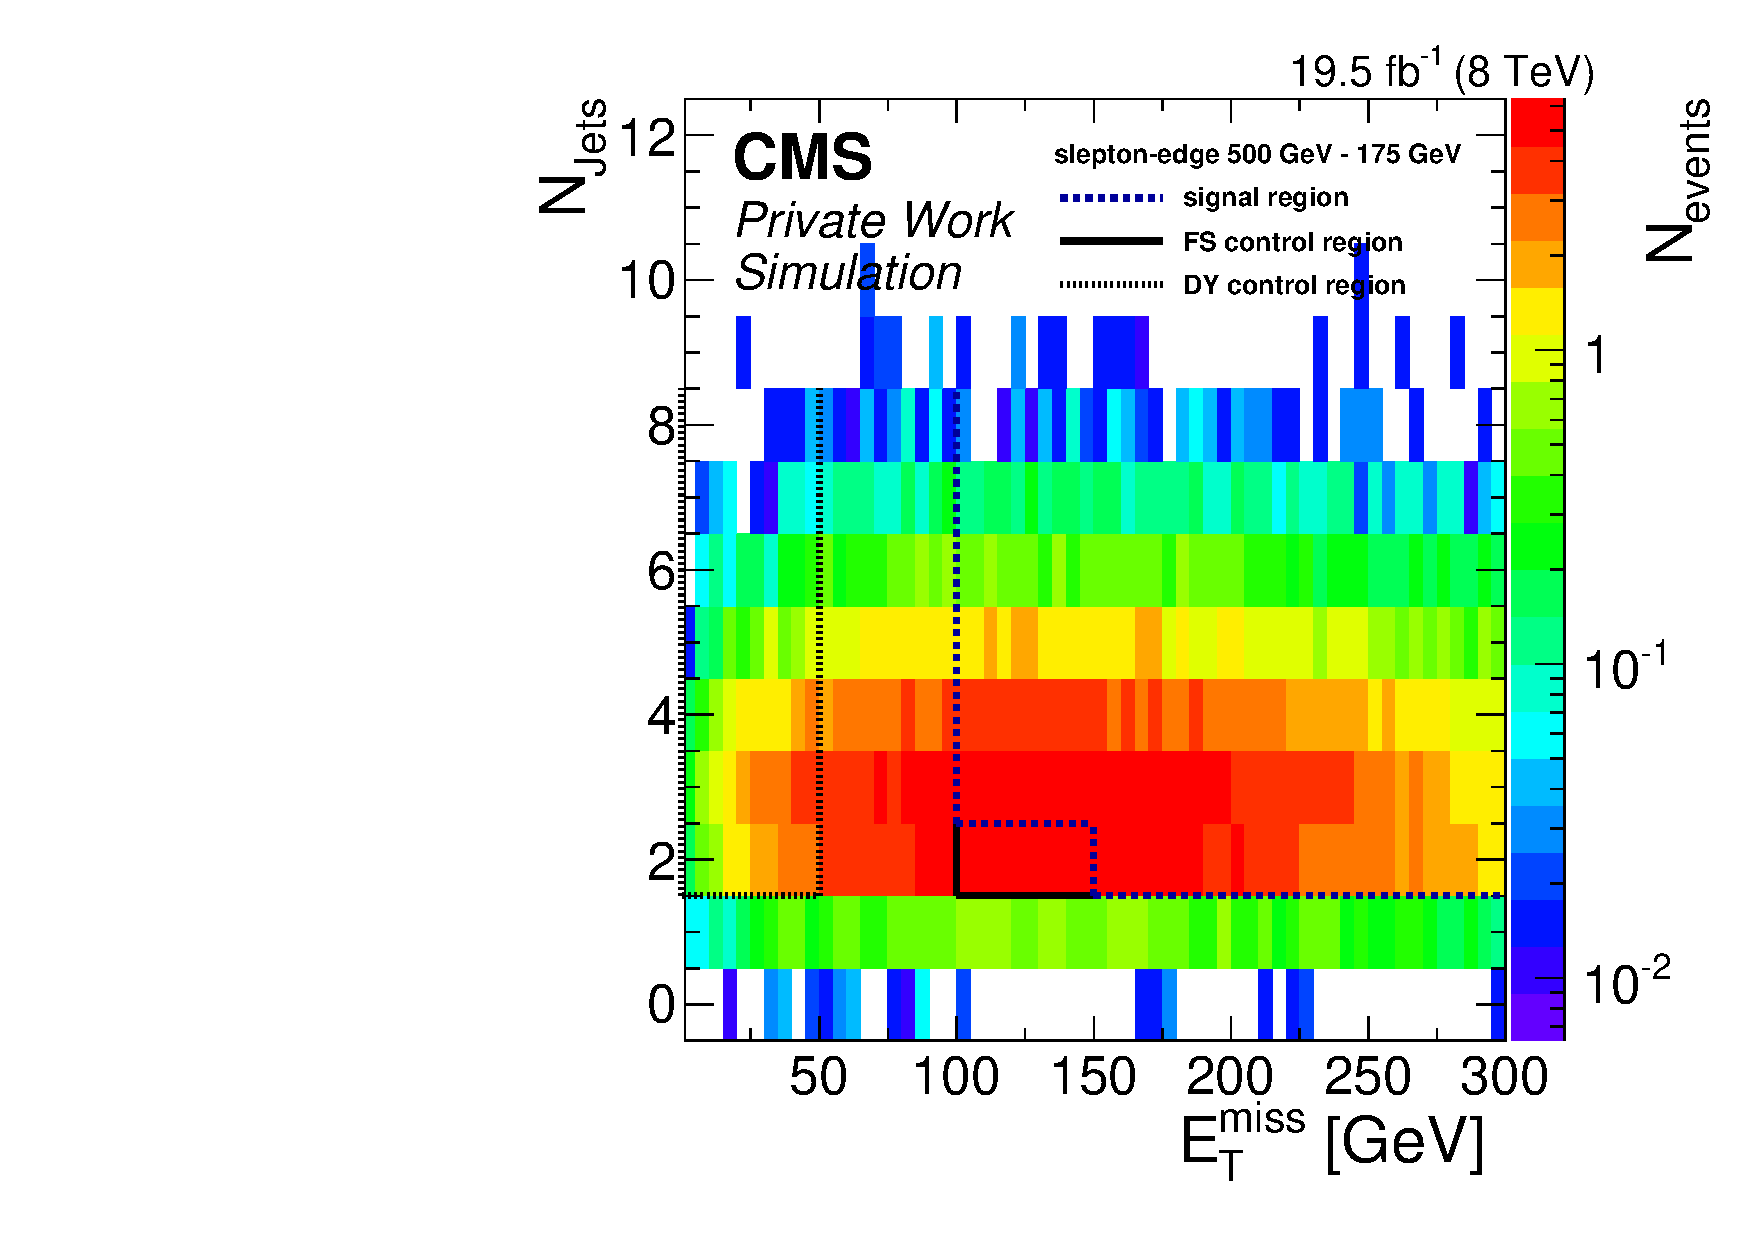
\includegraphics[width=\textwidth]{plots/SELECTION/metJetsScatter_SUSY_slepton_500_175.pdf}
\end{minipage}
\caption{Distribution of signal events with SF leptons in the \MET-$N_{jets}$ plane. Shown is one point from the fixed-edge model with $m_{\sbottom} = \unit{550}{\giga\electronvolt}$ and $m_{\secondchi} = \unit{275}{\giga\electronvolt}$ (left) and one from the slepton-edge model with $m_{\sbottom} = \unit{500}{\giga\electronvolt}$ and $m_{\secondchi} = \unit{175}{\giga\electronvolt}$ (right). The events are weighted according to their cross section and the size of the generated event sample, assuming an integrated luminosity of \lumi. The three regions defined in the plane are indicated by lines. The central and forward dilepton selection are combined.}
\label{fig:sigRegionSignal}
\end{figure}    

\subsection{Selection in \mll}
The analysis is performed using two different approaches. In a ``counting experiment'', described in section~\ref{sec:counting}, an excess in the number of observed events over the background expectation is sought in three regions of dilepton invariant mass \mll: low-mass ($\mathrm{20}< \mll < \unit{70}{\giga\electronvolt}$), on-\Z ($\mathrm{80}< \mll < \unit{101}{\giga\electronvolt}$) and high-mass ($\unit{120}{\giga\electronvolt} > \mll$). Figure~\ref{fig:sigMC} shows the \mll distribution in the central region for simulated SM backgrounds, which are shown separated into different physics processes. It can be seen that \ttbar is the dominant background in all three mass bins. For the on-\Z region also Drell--Yan backgrounds contribute significantly. The precise determination of these backgrounds from data are described in section~\ref{sec:backgrounds} and the results of the counting experiment are discussed in section~\ref{sec:counting}.

\begin{figure}[htbp]
\centering
\begin{minipage}[t]{0.49\textwidth}
  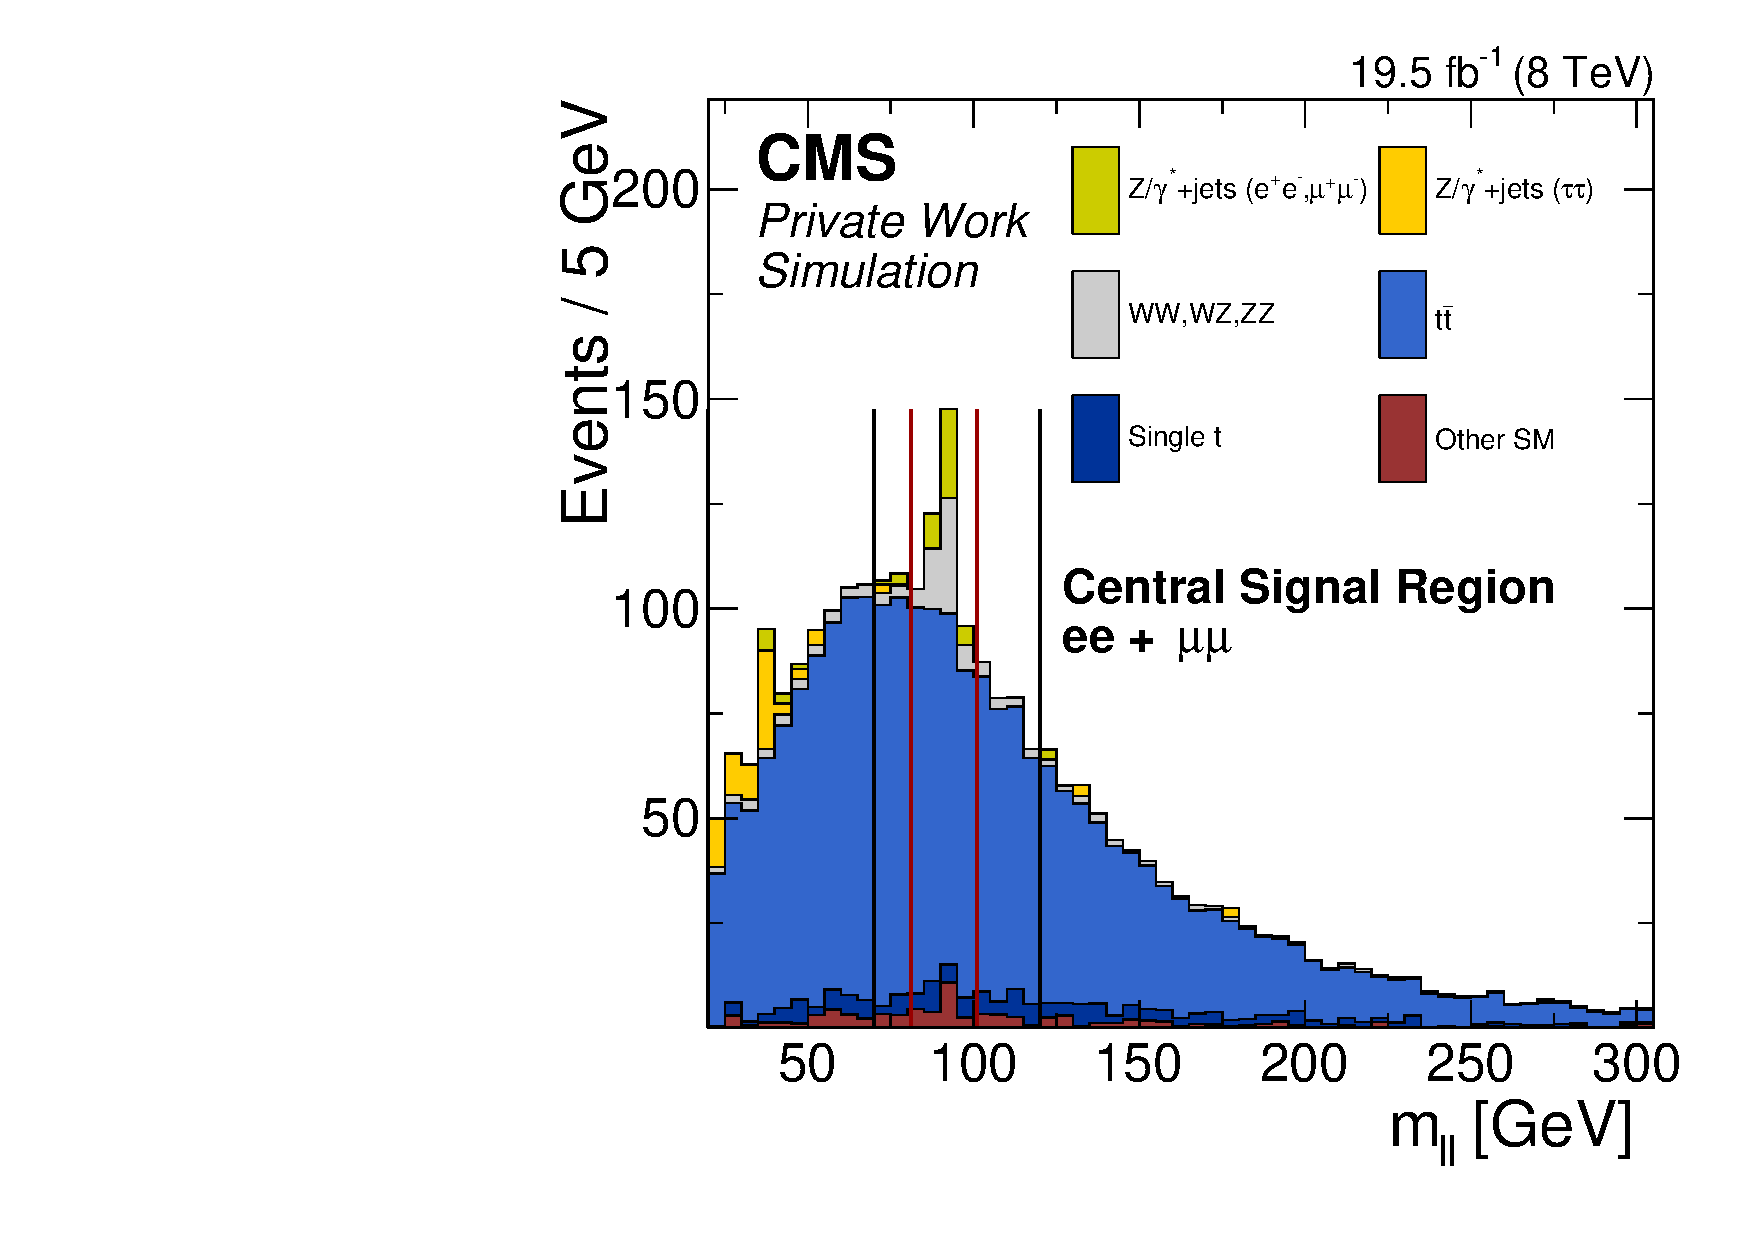
\includegraphics[width=\textwidth]{plots/SELECTION/SignalCentral_Mll_Full2012_SF_TopReweighted_MCOnly.pdf}
\end{minipage}
\begin{minipage}[t]{0.49\textwidth}
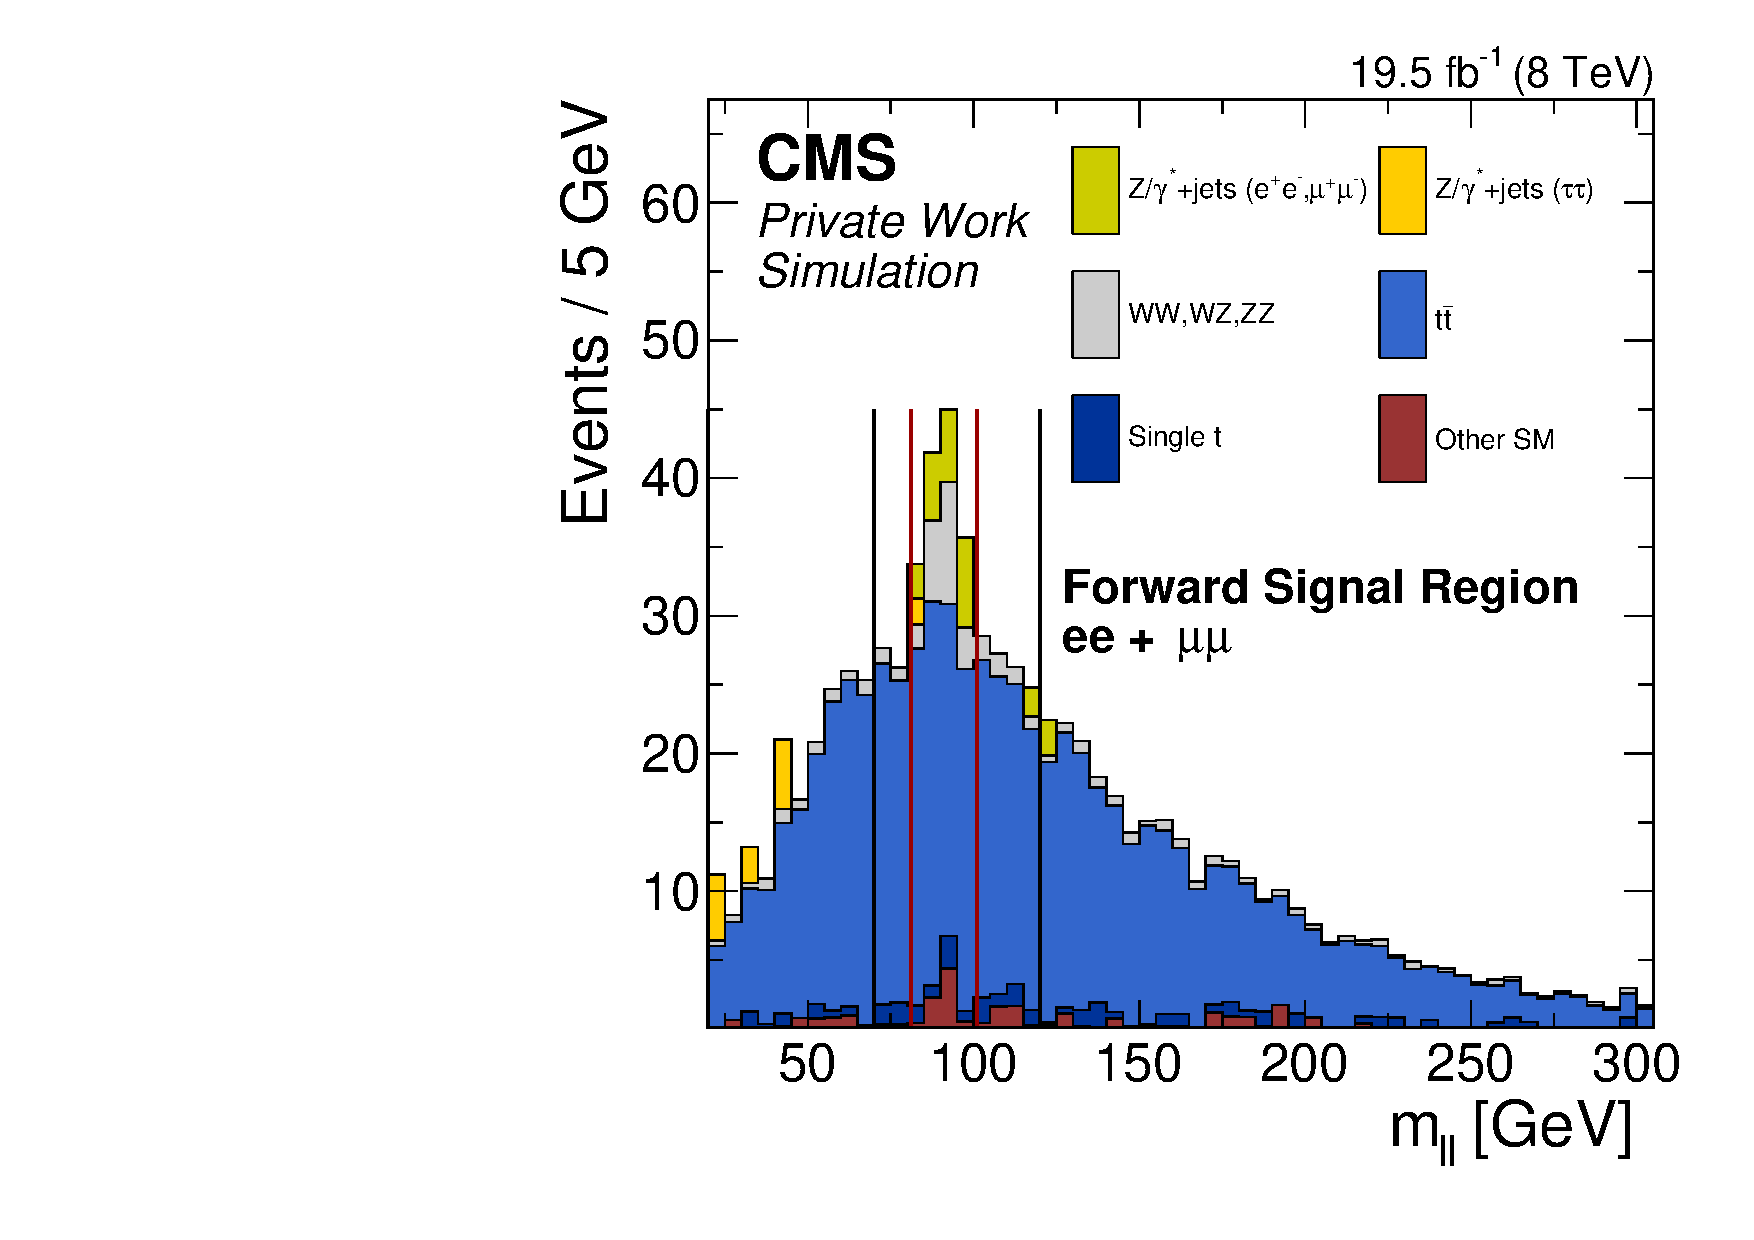
\includegraphics[width=\textwidth]{plots/SELECTION/SignalForward_Mll_Full2012_SF_TopReweighted_MCOnly.pdf}
\end{minipage}
\caption{Distribution of \mll in SM simulation in the signal region. The different background contributions are shown as stacked histogram. The distribution is normalized to \lumi. The red lines indicate the on-\Z region while the black lines show the boundaries of the low-mass and high-mass regions.}
\label{fig:sigMC}
\end{figure}

Additionally, a shape analysis is performed to directly search for edges in the \mll spectrum. Here the mass range $\mathrm{20}< \mll < \unit{300}{\giga\electronvolt}$ is studied. It is described in section~\ref{sec:fit}.

